\PassOptionsToPackage{numbers}{natbib}
\documentclass[a4paper,14pt,oneside,openany]{memoir}
\usepackage[left=30mm, top=20mm, right=15mm, bottom=20mm, nohead, nofoot]{geometry}
\usepackage[utf8]{inputenc}
\usepackage[english, russian]{babel}

\usepackage[T2A]{fontenc}

\usepackage{url}
\usepackage{booktabs}
\usepackage{amsfonts}
\usepackage{nicefrac}
\usepackage{microtype}
\usepackage{graphicx}
\usepackage{natbib}
\usepackage{doi}
\usepackage{amsmath}
\usepackage{amsthm}
\usepackage{bbm}
\usepackage{dsfont}

% Please add the following required packages to your document preamble:
 \usepackage{multirow}
 \usepackage[table,xcdraw]{xcolor}
% Beamer presentation requires \usepackage{colortbl} instead of \usepackage[table,xcdraw]{xcolor}


%%% Работа с русским языком
\usepackage{cmap}			 % поиск в PDF
\usepackage{mathtext} 		 % русские буквы в формулах
\usepackage[T2A]{fontenc}	 % кодировка
\usepackage[utf8]{inputenc}	 % кодировка исходного текста


%%% Пакеты для работы с математикой
\usepackage{amsmath,amsfonts,amssymb,amsthm,mathtools}
\usepackage{icomma}

%% Номера формул
%\mathtoolsset{showonlyrefs=true} % Показывать номера только у тех формул, на которые есть \eqref{} в тексте.
%\usepackage{leqno}               % Немуреация формул слева

%% Шрифты
\usepackage{euscript}	 % Шрифт Евклид
\usepackage{mathrsfs}    % Красивый матшрифт
\usepackage{bm}

%% Поля (геометрия страницы)
%\usepackage[left=3cm,right=2cm,top=2cm,bottom=2cm,bindingoffset=0cm]{geometry}

%% Русские списки
\usepackage{enumitem}
\makeatletter
\AddEnumerateCounter{\asbuk}{\russian@alph}{щ}
\makeatother


\pagestyle{plain}
%%% Работа с картинками
\usepackage{caption}
\captionsetup{justification=centering} % центрирование подписей к картинкам
\usepackage{graphicx}                  % Для вставки рисунков
\graphicspath{{images/}{images2/}}     % папки с картинками
\setlength\fboxsep{3pt}                % Отступ рамки \fbox{} от рисунка
\setlength\fboxrule{1pt}               % Толщина линий рамки \fbox{}
\usepackage{wrapfig}                   % Обтекание рисунков и таблиц текстом

%%% Работа с таблицами
\usepackage{array,tabularx,tabulary,booktabs} % Дополнительная работа с таблицами
\usepackage{longtable}                        % Длинные таблицы
\usepackage{multirow}                         % Слияние строк в таблице

%% Красная строка
\setlength{\parindent}{2em}

%% Интервалы
\linespread{1.2}
\usepackage{multirow}

%% TikZ
\usepackage{tikz}
\usetikzlibrary{graphs,graphs.standard}


%% Перенос знаков в формулах (по Львовскому)
%\newcommand*{\hm}[1]{#1\nobreak\discretionary{}{\hbox{$\mathsurround=0pt #1$}}{}}

%% дополнения
\usepackage{float}   % Добавляет возможность работы с командой [H] которая улучшает расположение на странице
\usepackage{gensymb} % Красивые градусы
\usepackage{caption} % Пакет для подписей к рисункам, в частности, для работы caption*

% подключаем hyperref (для ссылок внутри  pdf)

\hypersetup{
	colorlinks=true,
	linkcolor=black,
	filecolor=black,      
	urlcolor=black,
	pdfpagemode=FullScreen,
	citecolor=black
}


\usepackage[utf8]{inputenc}

%% Default fixed font does not support bold face
\DeclareFixedFont{\ttb}{T1}{txtt}{bx}{n}{12} %% for bold
\DeclareFixedFont{\ttm}{T1}{txtt}{m}{n}{12}  %% for normal

%% Custom colors
\usepackage{color}
\definecolor{deepblue}{rgb}{0,0,0.5}
\definecolor{deepred}{rgb}{0.6,0,0}
\definecolor{deepgreen}{rgb}{0,0.5,0}

\usepackage{listings}

%% Python style for highlighting
\newcommand\pythonstyle{\lstset{
		language=Python,
		basicstyle=\ttm,
		morekeywords={self},              %% Add keywords here
		keywordstyle=\ttb\color{deepblue},
		emph={MyClass,__init__},          %% Custom highlighting
		emphstyle=\ttb\color{deepred},    %% Custom highlighting style
		stringstyle=\color{deepgreen},
		frame=tb,                         %% Any extra options here
		showstringspaces=false
}}


% Python environment
\lstnewenvironment{python}[1][]
{
	\pythonstyle
	\lstset{#1}
}
{}

% Python for external files
\newcommand\pythonexternal[2][]{{
		\pythonstyle
		\lstinputlisting[#1]{#2}}}

% Python for inline
\newcommand\pythoninline[1]{{\pythonstyle\lstinline!#1!}}


%% Определения теорем и определений
\newtheorem{definition}{Определение}
\newtheorem{theorem}{Теорема}

%% Настройка документа
\setcounter{secnumdepth}{3}
  \setcounter{tocdepth}{3}

 % Начинаем нумерацию глав с 0 (для технических целей)
\renewcommand{\thechapter}{\arabic{chapter}} % Формат номера главы (1, 2, 3...)

% Специальная команда для ненумерованного введения
\newcommand{\introchapter}[1]{
	\chapter*{#1}
	\addcontentsline{toc}{chapter}{#1} % Добавляем в оглавление
	\markboth{#1}{#1} % Для колонтитулов
}

\AtBeginDocument{\selectlanguage{russian}}
\begin{document}


\begin{center}
	%% *название института*
	\large\textbf{Министерство образования и науки Российской Федерации \\
		Московский физико-технический институт (государственный
		университет)} \\
	\vspace{1cm}
	
	%% *факультет/физтех-школа*
	Физтех-школа прикладной математики и информатики \\
	
	%% *название базовой кафедры и лаборатории*
	%% в случае ненадобности можно удалить
	Кафедра алгоритмов и технологии программирования \\
	
	
	\vspace{2em}
	
	Выпускная квалификационная работа магистра
\end{center}

\begin{center}
	\vspace{\fill}
	%% *название вашей работы*
	\LARGE{Нейросетевые модели анализа выживаемости для решения задачи предсказания оттока абонентов}
	
	\vspace{\fill}
\end{center}


\begin{flushright}
	\textbf{Автор:} \\
	Студент М05-313а группы \\
	Батарин Егор Владиславович \\
	\vspace{2em}
	\textbf{Научный руководитель:} \\
	Джумакаев Тимур Казбекович \\
	
\end{flushright}

\vspace{2em}

\begin{center}
	%% *лого*
	
\includegraphics[width=100 pt]{../figures/MIPT_logo.jpg}\\
	Москва \the\year{}
\end{center}

% выключаем отображение номера для этой страницы (титульник)
\thispagestyle{empty}

\newpage


	
	
	\begin{abstract}
		%\thispagestyle{plain}
		\begin{center}
			\large{Нейросетевые модели анализа выживаемости для решения задачи предсказания оттока абонентов} \\
			\large\textit{Батарин Егор Владиславович} \\[1 cm]
		\end{center}
		
	В работе решается задача прогнозирования оттока абонентов компании Мегафон. Проведен анализ существующих решений из моделей анализа выживаемости, кратко описаны их отличия и проведены сравнения данных моделей на задаче оттока клиентов Мегафона. \\
		
	 Задача рассматривается как многоклассовая классификация, где в качестве меток класса выбраны факты оттока в будущие месяцы и факт отсутствия оттока в эти месяцы. Предлагаются различные подходы к решению задачи, как классические подходы: градиентный бустинг и модель Кокса, так и более современные подходы, связанные с применением методов глубокого обучения в моделях выживаемости. Проводится сравнение различных подходов с точки зрения принятых в работе критериев качества.\\
	 
	 В рамках работы была разработана модель, отличающаяся от предыдущих использованием временных рядов векторов признаков. Основная новизна работы заключается в использовании специфической функции потерь. В работе доказывается свойство добавки к функции потерь. Модель, разработанная в данной работе, показала более высокие результаты по сравнению с другими моделями в плане более низкой потери качества на "сжатом" признаковом описании и более высоким $C$-индексом.\\

		
		
		
	\end{abstract}
	
\newpage
	
	\tableofcontents


\introchapter{Введение}

Данная работа посвящена решению задачи прогнозирования оттока в контексте телекоммуникационной отрасли в рамках проекта компании Мегафон. Данная задача позникает в большом количестве различных индустрий и для ее решения используются разные подходы. \cite{Ahn2020}. Среди всех таких подходов, включающих в себя разные современные методы машинного обучения (SVM, Random Forest, Gradient Boosting) основным направлением исследований для решения данной задачи был выбран анализ выживаемости. 

Классической работой по анализу выживаемости является модель пропорциональных рисков \cite{Cox1972}. В настоящее время появилось много новых подходов, так или иначе задействующих глубокое обучение \cite{Wiegrebe2024}. Эти подходы расширяют классические модели анализа выживаемости, позволяя обойти некоторые предположения о данных, которые на практике редко выполняются, например, предположение о пропорциональности рисков. Все модели анализа выживаемости можно разделить на две категории с зависимости от того, считается ли время непрерывным или дискретным. Поскольку специфика проекта Мегафона требует рассмотрения дискретного времени, то именно такой случай фигурирует в постановке задачи. 

Одной из известных дискретных моделей выживаемости является модель DeepHit \cite{Lee2018}, являюшейся одной из основных для сравнения в дискретной постановке задачи. 

Одним из самых распространенных подходов к задаче является градиентый бустинг \cite{Ahmad2019}.  В данной работе в качестве базового подхода рассматривается категориальный бустинг от компании Яндекс \cite{Dorogush2018}. Он получил большое распространение на российском рынке, поэтому исследуемые в работе подходы, основанные на анализе выживаемости, сравниваются с CatBoost.

В работе используются внутренние датасеты компании Мегафон, собранные на основе данных в КХД. В роли критериев качества модели выступают метрики Precision, Recall, F1, вычисленные при различных вероятностных порогах - числах, позволяющих перевести вероятности классов в метки классов.


\setcounter{chapter}{0}




\chapter{Постановка задачи}

\section{Общая постановка задачи анализа выживаемости}

В дискретном случае время имеет вид $\mathcal{T}=\{0,\ldots,T_{\max}\}$, где $T_{\max}$ - это максимальный горизонт предсказания (например, максимально возможное время жизни абонента). В любой их этих моментов может произойти событие $\mathcal{K}=\{\emptyset,1,\cdots,K\}$, где все события $\{1,\cdots,K\}$ соответствуют факту оттока по одной из $K$ возможных причин в некоторый момент времени $\tau$, а событие $\emptyset$ означает факт правого цензурирования - информация о том, что отток произойдет не раньше того времени $\tau$, когда произошло цензурирование, но точно неизвестно когда именно. Для каждого момента времени, таким образом, мы можем написать $\tau^i=\min(T^i,C^i)$, где $T^{i}\in\mathcal{T}$ - это времена наступлений одного из событий $\{1,\cdots,K\}$, а $C^{i}\in\mathcal{T}$ соответствует право-цензурированным событиям $\emptyset$. Имея в распоряжении информацию о произошедших событиях (включая цензурирования) $\{\tau^{i},k^{i})\}_{i=1}^{N}$ и некоторую дополнительную информацию о признаках абонентов, мы хотим научиться предсказывать вероятности наступления события из $\mathcal{K}$ в будущем. В зависимости от того, рассматриваем ли мы признаки абонентов только в один момент времени или рассматриваем для каждого абонента временной ряд соотвествующих ему признаков, будет немного различаться математическая постановка задачи. 

Непрерывный случай отличается от дискретного тем, что время представляет из себя отрезок 

\section{C-индекс и его связь с ранжированием абонентов}


Специфичным для анализа выживаемости критерием качества является C-индекс (concordante index) \cite{Alabdallah2022}, являющийся аналогом широкого известного критерия качества AUC. Дадим его строгое определение: 

\begin{definition}
Пусть для пары абонентов $(i,j)$ определены $\tau_i$  < $\tau_j$ - моменты времени (возможно, цензурированные), $\delta_i$ - индекс цензурирования, равный $0$, если $\tau_i$ право-цензурировано и $1$ - в противном случае. Также обозначим через $\hat{F}_{k,i}$ и $\hat{F}_{k,j}$ вероятности оттока до момента по событию $k$ времени $\tau_i$ для абонентов $i$ и $j$ соответственно (оцененные моделью функции распределения). Тогда C-индекс определяется следующим образом:

$$C\text{-}index =
\frac{
	\sum\limits_{i,j} \mathbf{1}_{\tau_i < \tau_j} \cdot \mathbf{1}_{\hat{F}_{k,i} > \hat{F}_{k,j}} \cdot \delta_i
}{
	\sum\limits_{i,j} \mathbf{1}_{\tau_i < \tau_j} \cdot \delta_i
}$$	
\end{definition}

Нам также понадобится определение верно упорядоченной пары абонентов: 

\begin{definition}
Пара абонентов $(i,j)$ считается верно упорядоченной (отранжированной), если для оцененных моделью функций распределений $\hat{F}_{k,i}$ и $\hat{F}_{k,j}$ выполнено неравенство: 

$$ \hat{F}_{k,i}(\tau_i ) >  \hat{F}_{k,j}(\tau_i ) $$ 
\end{definition}





 Он численно равен доле пар абонентов, которые модель верно упорядочила. 

Этот индекс отражает то разумное требование к моделям выживаемости, которое заключается в том, что если абонент $i$ оттекает раньше абонента $j$, то оцениваемая моделью вероятность его оттока до момента его фактического оттока будет больше, чем аналогичная вероятность для $j$ абонента, рассматриваемая для того же момента времени - фактического оттока $i$-ого абонента. 

\section{Постановка с одним вектором-признаком}

В данной модели предполагается, что абонент полностью описывается вектором $\bold{x} \in X$, соответственно обучающая выборка имеет вид $\mathcal{D}=\{(\mathbf{x}^{(i)},\tau^{(i)},k^{(i)})\}_{i=1}^N$, вероятности нецензурированных событий $k^* \neq \emptyset $ имеют вид $P(\tau=\tau^*,k=k^*|\mathbf{x}=\mathbf{x}^*)$, а функция распределения имеет вид:

\begin{align}
	F_{k^*}(t^*|\mathbf{x}^*) &= P(\tau\leq t^*,k=k^*|\mathbf{x}=\mathbf{x}^*) 
	= \sum_{\tau^*=0}^{t^*} P(\tau=\tau^*,k=k^*|\mathbf{x}=\mathbf{x}^*).
\end{align}




\section{Поставнока в временным рядом векторов-признаков}

Эта модель является расширением предыдущей и для каждого абонента $i$ в ней рассматривается уже не единственный вектор-признак $\bold{x}_i$, а временной ряд векторов-признаков: 
$$\mathcal{X}^i(t)=\{\mathbf{x}^i(t_j^i):0\leq t_j^i\leq t\mathrm{~for~}j=1,\cdots,J^i\}$$, где $\mathbf{x}^i(t_j)$ - это вектор признак $i$-ого абонента, замеренный в момент времени $t_j$ и равный $\mathbf{x}_j^i=[x_{j,1}^{i},\cdots,x_{j,d_{r}}^{i}]$. Кроме того, в этой модели для каждого абонента $i$ вводится набор векторов-флагов $\mathrm{M}^i=\{\mathrm{m}_1^i,\cdots,\mathrm{m}_{J^i}^i\}$, $\mathbf{m}_j^i=[m_{j,1}^i,\cdots,m_{j,d_x}^i]$, которые сигнализируют о пропущенных значениях: $m_{j,d}^{i}=1$ тогда и только тогда, когда $x_{j,d}^{i}$ пропущено, иначе $m_{j,d}^{i}=0$. Напоследок, вводится последовательность векторов временных интервалов между замерами времени $\Delta_i = \{\delta_{1}^{i},\delta_{2}^{i}\cdots,\delta_{J^{i}}^{i}\}$, где $\delta_{j}^{i}=t_{j+1}^{i}-t_{j}^{i}$ для всех $1\leq j<J^{i}$ и $\delta_{J^i}^i=0$. В итоге получается обучающая выборка: $\mathcal{D}=\{(\mathbf{X}^{i},\mathbf{M}^{i},\Delta^{i},\tau^{i},k^{i})\}_{i=1}^{N}$.

\chapter{Существующие подходы в анализе выживаемости}

\section{Непрерывные модели выживаемости}

\section{Оценка Каплана--Майера}

Оценка Каплана--Майера~\cite{Kaplan1958} (иногда также называемая оценкой произведения лимита, англ. \textit{product-limit estimator}) представляет собой непараметрический метод оценки функции выживания $S(t)$, которая определяет вероятность того, что событие не произойдёт до момента времени $t$, то есть $S(t) = \mathbb{P}(T > t)$. Этот метод широко используется в анализе выживаемости, особенно в случаях, когда данные частично цензурированы.

Пусть дана выборка из $N$ объектов. Для каждого наблюдения $i \in \{1, 2, \dots, N\}$ известны:
\begin{itemize}
	\item время наблюдения $\tau^i \in \mathbb{R}_+$ — либо время наступления события, либо момент последнего контакта;
	\item индикатор события $\delta^i \in \{0, 1\}$, где
	\begin{itemize}
		\item $\delta^i = 1$ означает, что событие (например, отток, смерть, выход из системы и т.д.) произошло в момент $\tau^i$;
		\item $\delta^i = 0$ означает, что наблюдение было право-цензурировано, то есть объект «выпал» из исследования по другим причинам, и мы не знаем, когда у него наступит событие.
	\end{itemize}
\end{itemize}

Предположим, что в выборке имеется $K$ уникальных моментов времени $t_1 < t_2 < \dots < t_K$, в которые происходили события (т.е. $\delta^i = 1$ для некоторых $i$ и $\tau^i = t_k$). Обозначим:
\begin{itemize}
	\item $d_k$ — количество событий, произошедших в момент $t_k$;
	\item $n_k$ — количество объектов, находившихся под наблюдением непосредственно перед моментом $t_k$, то есть таких $i$, что $\tau^i \geq t_k$.
\end{itemize}

Тогда оценка Каплана--Майера для функции выживания имеет вид:

\begin{equation}
	\hat{S}(t) = \prod_{t_k \leq t} \left(1 - \frac{d_k}{n_k} \right),
\end{equation}

где произведение берётся по всем моментам времени $t_k$, не превосходящим $t$.

Интуитивно эта формула отражает идею пошагового снижения вероятности выживания: на каждом шаге учитывается вероятность «выжить» после очередного события, при этом цензурированные данные не учитываются в $d_k$, но входят в $n_k$, пока остаются под наблюдением.

\vspace{1em}
\noindent
\textbf{Пример:} Если из 10 объектов на первом шаге событие происходит у 1, то вероятность выживания после первого шага — $1 - \frac{1}{10} = 0.9$. На следующем шаге, если осталось 9 объектов и снова у одного происходит событие, то следующий множитель — $1 - \frac{1}{9}$, и так далее.

\vspace{1em}
\noindent
\textbf{Свойства оценки:}
\begin{itemize}
	\item $\hat{S}(t)$ представляет собой ступенчатую функцию, убывающую по мере увеличения $t$.
	\item Оценка не требует предположений о виде распределения времени до события.
	\item Метод устойчив к право-цензурированным данным: такие наблюдения учитываются при подсчёте риска, но не влияют непосредственно на снижение $\hat{S}(t)$.
\end{itemize}

\vspace{1em}
\noindent
\textbf{Связь с теоремой Гливенко--Кантелли:} Можно отметить, что оценка Каплана--Майера является аналогом эмпирической функции распределения (ЭФР) в условиях цензурирования. В классическом случае (без цензурирования) сходимость эмпирической функции распределения к истинной описывается теоремой Гливенко--Кантелли, согласно которой:

\begin{equation}
	\sup_{t} |\hat{F}_n(t) - F(t)| \xrightarrow[n \to \infty]{} 0 \quad \text{почти наверное}.
\end{equation}

Аналогично, оценка Каплана--Майера также является состоятельной: она сходится к истинной функции выживания $S(t)$ при увеличении объёма выборки, даже в присутствии цензурирования. Эта сходимость была доказана в рамках расширения классических результатов теории эмпирических процессов на случай неполных данных.

\vspace{1em}
\noindent
\textbf{Ограничения метода:}
\begin{itemize}
	\item Оценка Каплана--Майера не учитывает признаков (факторов) объектов, т.е. она одинаково трактует все наблюдения, независимо от индивидуальных характеристик $\mathbf{x}^i$.
	\item Метод не позволяет строить индивидуализированные предсказания выживания (например, вероятность выживания конкретного пациента).
	\item При большом числе возможных моментов времени (особенно при малом размере выборки) оценка может быть «шумной» и требовать сглаживания.
\end{itemize}

Несмотря на эти ограничения, оценка Каплана--Майера остаётся важным инструментом для первичного анализа и визуализации данных выживания, а также служит основой для многих более сложных моделей (например, стратифицированных анализов или моделей пропорциональных рисков Кокса).


\subsection{Модель пропорциональных рисков Кокса}

Модель пропорциональных рисков, предложенная Дэвидом Коксом в 1972 году~\cite{Cox1972}, представляет собой полупараметрическую модель анализа выживаемости. Её основное достоинство — возможность моделировать влияние признаков на риск наступления события, не делая предположений о конкретной форме временного распределения базовой функции риска.

\vspace{1em}
\noindent
\textbf{Функция риска.} Основная идея модели Кокса заключается в предположении, что условная функция риска $h(t|\mathbf{x})$ для объекта с признаковым вектором $\mathbf{x} \in \mathbb{R}^d$ может быть представлена в виде:

\begin{equation}
	h(t|\mathbf{x}) = h_0(t) \cdot \exp(\mathbf{x}^\top \boldsymbol{\beta}),
\end{equation}

где:
\begin{itemize}
	\item $h(t|\mathbf{x})$ — функция риска, т.е. мгновенная вероятность наступления события в момент $t$ при условии, что оно ещё не произошло;
	\item $h_0(t)$ — \textbf{базовая функция риска}, общая для всех наблюдений, отражающая как меняется риск во времени без учёта признаков;
	\item $\boldsymbol{\beta} \in \mathbb{R}^d$ — вектор параметров модели, определяющий влияние каждого признака на риск.
\end{itemize}

Базовая функция $h_0(t)$ не параметризуется явно, что делает модель Кокса полупараметрической: в отличие от полностью параметрических моделей (например, экспоненциальной или вейбулловской), здесь не предполагается форма распределения времени до события. Вся параметрическая часть заключается в оценке коэффициентов $\boldsymbol{\beta}$.

\vspace{1em}
\noindent
\textbf{Интерпретация.} Благодаря экспоненциальной форме зависимость между признаками и риском является мультипликативной. В частности, отношение рисков двух объектов с признаками $\mathbf{x}_1$ и $\mathbf{x}_2$ не зависит от времени и вычисляется как:

\begin{equation}
	\frac{h(t|\mathbf{x}_1)}{h(t|\mathbf{x}_2)} = \exp\left((\mathbf{x}_1 - \mathbf{x}_2)^\top \boldsymbol{\beta}\right).
\end{equation}

Это свойство называется \textit{пропорциональностью рисков} и составляет основное допущение модели.

\vspace{1em}
\noindent
\textbf{Функция выживания.} Поскольку функция риска $h(t|\mathbf{x})$ связана с функцией выживания $S(t|\mathbf{x})$ через следующее соотношение:

\begin{equation}
	S(t|\mathbf{x}) = \exp\left(-\int_0^t h(u|\mathbf{x}) \, du \right),
\end{equation}

в модели Кокса функция выживания для объекта с признаками $\mathbf{x}$ имеет вид:

\begin{equation}
	S(t|\mathbf{x}) = S_0(t)^{\exp(\mathbf{x}^\top \boldsymbol{\beta})},
\end{equation}

где $S_0(t)$ — функция выживания, соответствующая базовой функции риска $h_0(t)$. Таким образом, влияние признаков на выживаемость также проявляется через экспоненту: чем больше значение скалярного произведения $\mathbf{x}^\top \boldsymbol{\beta}$, тем быстрее убывает $S(t|\mathbf{x})$.

\vspace{1em}
\noindent
\textbf{Оценка параметров.} Коэффициенты $\boldsymbol{\beta}$ оцениваются путём максимизации так называемой \textbf{частичной функции правдоподобия} (\textit{partial likelihood}). Эта функция учитывает порядок наступления событий, но игнорирует форму $h_0(t)$:

\begin{equation}
	\mathcal{L}(\boldsymbol{\beta}) = \prod_{i:\delta^i=1} \frac{\exp(\mathbf{x}^{(i)\top} \boldsymbol{\beta})}{\sum_{j:\tau^j \geq \tau^i} \exp(\mathbf{x}^{(j)\top} \boldsymbol{\beta})},
\end{equation}

где произведение берётся по всем наблюдениям $i$, в которых событие действительно произошло ($\delta^i = 1$), а сумма в знаменателе вычисляется по \textbf{множеству риска} в момент времени $\tau^i$, включающем все объекты, ещё находившиеся под наблюдением к этому моменту.

\vspace{1em}
\noindent
Частичная правдоподобие удобно тем, что позволяет обойти оценку $h_0(t)$ и сфокусироваться на коэффициентах $\boldsymbol{\beta}$, которые описывают связь между признаками и риском.

\vspace{1em}
\noindent
\textbf{Свойства и достоинства:}
\begin{itemize}
	\item Модель Кокса обладает \textbf{высокой интерпретируемостью}. Коэффициенты $\beta_k$ можно трактовать как логарифмы относительных рисков: увеличение $k$-го признака на 1 увеличивает риск в $\exp(\beta_k)$ раз.
	\item Отсутствие предположений о виде функции риска $h_0(t)$ делает модель гибкой и пригодной в широком диапазоне задач.
	\item В модели можно использовать стратификацию, регуляризацию (например, L1 или L2) и расширения для работы с временными ковариатами.
\end{itemize}

\vspace{1em}
\noindent
\textbf{Ограничения модели:}
\begin{itemize}
	\item Основное допущение — \textit{пропорциональность рисков} — не всегда выполняется. Если реальные риски пересекаются, модель Кокса может давать некорректные выводы.
	\item Модель плохо справляется с \textbf{нелинейными зависимостями} между признаками и риском без дополнительного преобразования признаков.
	\item При высокоразмерных данных (когда количество признаков сравнимо или превышает количество наблюдений) модель склонна к переобучению без регуляризации.
	\item Она не позволяет напрямую предсказывать распределение времени до события $T$, а только функцию риска или выживания.
\end{itemize}

\vspace{1em}
\noindent
Несмотря на ограничения, модель Кокса остаётся одной из ключевых моделей в анализе выживаемости, активно используется в медицине, биостатистике, социологии и других науках, где важно учитывать влияние признаков на риск наступления события во времени.


\subsection{DeepSurv}

DeepSurv \cite{Katzman2018} — это нейросетевое расширение модели Кокса. Вместо линейной зависимости $\mathbf{x}^\top \boldsymbol{\beta}$ используется произвольная нелинейная функция, моделируемая нейросетью $f_\theta(\mathbf{x})$:

\begin{equation}
	h(t|\mathbf{x}) = h_0(t) \cdot \exp(f_\theta(\mathbf{x})).
\end{equation}

Модель обучается аналогично классической модели Кокса — путём максимизации частичной функции правдоподобия:

\begin{equation}
	\mathcal{L}(\theta) = -\sum_{i:\delta^i=1} \left[ f_\theta(\mathbf{x}^i) - \log \sum_{j:\tau^j \geq \tau^i} \exp(f_\theta(\mathbf{x}^j)) \right].
\end{equation}

Таким образом, DeepSurv сохраняет достоинства модели Кокса (работа с цензурированными данными), но благодаря использованию нейросетей способна учитывать сложные нелинейные зависимости между признаками и риском.

\section{Дискретные модели выживаемости}

\subsection{Nnet-survival}

Nnet-survival \cite{Gensheimer2019} — это дискретная нейросетевая модель, в которой время разделяется на интервалы $[0, t_1), [t_1, t_2), \dots, [t_{M-1}, t_M)$, и на каждом из них предсказывается условная вероятность наступления события.

Модель предсказывает условную вероятность $q_m = P(T \in [t_{m-1}, t_m) \mid T \geq t_{m-1}, \mathbf{x})$ с помощью softmax-выхода нейросети. Далее рассчитывается функция выживания:

\begin{equation}
	\hat{S}(t_m|\mathbf{x}) = \prod_{l=1}^{m} (1 - q_l).
\end{equation}

Функция распределения, в свою очередь:

\begin{equation}
	\hat{F}(t_m|\mathbf{x}) = 1 - \hat{S}(t_m|\mathbf{x}).
\end{equation}

Функция потерь имеет вид отрицательного логарифма правдоподобия:

\begin{equation}
	\mathcal{L} = -\sum_{i=1}^N \log P(\tau^i, \delta^i|\mathbf{x}^i),
\end{equation}

где в зависимости от того, цензурировано наблюдение или нет, вероятность имеет разный вид (используется либо $q_m$, либо $\hat{S}(t_m|\mathbf{x}^i)$).

Модель является более гибкой, чем классические методы, и хорошо работает при большом числе наблюдений и цензурировании, однако требует выбора разбиения времени.

\subsection{PMF (Probability Mass Function)}

PMF-модель  подходит для многоклассовой дискретной предсказательной задачи. Модель предсказывает полную функцию распределения вероятностей событий по времени:

\begin{equation}
	\mathbf{p} = [p_1, p_2, \ldots, p_T], \quad \sum_{t=1}^T p_t = 1,
\end{equation}

где $p_t = P(T = t \mid \mathbf{x})$ — вероятность наступления события в момент $t$.

Функция выживания тогда записывается как

\begin{equation}
	\hat{S}(t|\mathbf{x}) = \sum_{j=t+1}^T p_j.
\end{equation}

А функция распределения:

\begin{equation}
	\hat{F}(t|\mathbf{x}) = \sum_{j=1}^t p_j.
\end{equation}

Функция потерь — логарифмическое правдоподобие, аналогично Nnet-survival, но с прямым использованием вероятностей $p_t$:

\begin{equation}
	\mathcal{L} = -\sum_{i=1}^N \left[
	\delta^i \cdot \log p_{\tau^i}^{(i)} + (1 - \delta^i) \cdot \log \hat{S}(\tau^i|\mathbf{x}^i)
	\right].
\end{equation}

Преимуществом модели является простота и интерпретируемость, а также прямая оценка распределения времени до события. Однако, как и в Nnet-survival, требуется дискретизация времени, что может снизить точность при неудачном разбиении.

\subsection{Модель DeepHit}

Поскольку теоретическая функция распределения неизвестна, то рассматривается ее оценка 
\begin{equation}
	\begin{aligned}
		\hat{F}_{k^*}(\tau^*|\mathbf{x}^*)=\sum_{m=0}^{\tau^*}o_{k,m}^*
	\end{aligned}
\end{equation}

на основе ответов модели DeepHit: $\mathbf{o}=[o_{1,1},\cdots,o_{1,T_{\max}},\cdots,o_{K,1},\cdots,o_{K,T_{\max}}]$, где $o_{k,\tau}$ - оценка моделью DeepHit вероятности того, что событие оттока $k$ произойдет в момент времени $\tau$.

В качестве функции потерь используется сумма двух слагаемых $\mathcal{L}_{\mathrm{Total}}=\mathcal{L}_1+\mathcal{L}_2$, в которой первое слагаемое имеет вид: 
\begin{equation}
	\begin{aligned}
		\mathcal{L}_{1} & = -\sum_{i=1}^N \left[\mathbbm{1}(k^{(i)}\neq\emptyset)\cdot\log\left(y_{k^{(i)},\tau^{(i)}}^{(i)}\right)  + \mathbbm{1}(k^{(i)}=\emptyset)\cdot\log\left(1-\sum_{k=1}^K\hat{F}_k(\tau^{(i)}|\mathbf{x}^{(i)})\right)\right]
	\end{aligned}
\end{equation}

и оно отвечает за логарифмическое правдоподобие, а второе слагаемое имеет вид: 
\begin{equation}
	\begin{aligned}
		\mathcal{L}_2=\sum_{k=1}^K\alpha_k\cdot\sum_{i\neq j}A_{k,i,j}\cdot\eta\left(\hat{F}_k(\tau^{(i)}|\mathbf{x}^{(i)}),\hat{F}_k(\tau^{(i)}|\mathbf{x}^{(j)})\right)
	\end{aligned}
\end{equation}

где $A_{k,i,j} = \mathbb{I}(k^{(i)}=k,\tau^{(i)}<\tau^{(j)})$ - индикатор того, что событие $k$ наступает для $j$-ого абонента позже, чем для $i$-ого и функция
$\eta(x,y)=\exp\left(\frac{-(x-y)}{\sigma}\right)$. 

\chapter{Описание подхода, разработанного в данной работе}


\section{Решение задачи для временного ряда векторов-признаков}

Теоретическая функция распределения в нашей модели принимает вид:

\begin{equation}
	\begin{aligned}
		F_{k^{*}}(\tau^{*}|\mathcal{X}^{*}) & = P(T\leq\tau^{*},k=k^{*}|\mathcal{X}^{*},T>t_{J^{*}}^{*}) = \\
		& =\sum_{\tau\leq\tau^*}P(T=\tau,k=k^*|\mathcal{X}^*,T>t_{J^*}^*).
	\end{aligned}
\end{equation}

Теоретическая функция выживания вычисляется следующим образом:

\begin{equation}
	\begin{aligned}
		S(\tau^{*}|\mathcal{X}^{*}) & = 
		P(T>\tau^*|\mathcal{X}^*,T>t_{J^*}^*) =\\
		& =1-\sum_{k\neq\emptyset}F_k(\tau^*|\mathcal{X}^*)
	\end{aligned}
\end{equation}

Поскольку теоретические функции неизвестны, мы можем пользоваться только оценочными. Оценочная функция распределения выражается через ответы модели:
\begin{equation}
	\begin{aligned}
		\hat{F}_{k^*}(\tau^*|\mathcal{X}^*)=\frac{\sum_{t_{J^*}^*<\tau\leq\tau^*}o_{k^*,\tau}^*}{1-\sum_{k\neq\emptyset}\sum_{n\leq t_{J^*}^*}o_{k,n}^*}
	\end{aligned}
\end{equation}

Функция потерь состоит из трех частей: $\mathcal{L}_{\mathrm{Total}}=\mathcal{L}_1+\mathcal{L}_2+\mathcal{L}_3$. Слагаемые $\mathcal{L}_1$ и $\mathcal{L}_2$ аналогичны соответствующим слагаемым из модели DeepHit и имеют вид: 

\begin{equation}
	\begin{aligned}
		\mathcal{L}_{1} & =-\sum_{i=1}^N\left[\mathbbm{1}(k^i\neq\emptyset)\cdot\log\Big(\frac{o_{k^i,\tau^i}^i}{1-\sum_{k\neq\emptyset}\sum_{n\leq t_{Ji}^i}o_{k,n}^i}\Big)\right] \\
		& +\mathbbm{1}(k^i=\emptyset)\cdot\log\biggl(1-\sum_{k\neq\emptyset}\hat{F}_k(\tau^i|\mathcal{X}^i)\biggr)\biggr]
	\end{aligned}
\end{equation}

\begin{equation}
	\begin{aligned}
		\mathcal{L}_2=\sum_{k=1}^K\alpha_k\sum_{i\neq j}A_{kij}\cdot\eta\left(\hat{F}_k(s^i+t_{J^i}^i|\mathcal{X}^i),\hat{F}_k(s^i+t_{J^j}^j|\mathcal{X}^j)\right)
	\end{aligned}
\end{equation}
, где $s^i=\tau^i-t_{J^i}^i$, $A_{kij}=\mathbbm{1}(k^i=k,s^i<s^j)$ , $\eta(a,b)=\exp\left(-\frac{a-b}{\sigma}\right)$


Третье слагаемое в общей функции потерь является новым и отвечает за регуляризацию временных рядов: 

\begin{equation}
	\begin{aligned}
		\mathcal{L}_3=\beta\cdot\sum_{i=1}^N\sum_{j=0}^{J^i-1}\sum_{d\in\mathcal{I}}(1-m_{j+1,d}^i)\cdot\zeta(x_{j+1,d}^i,y_{j,d}^i)	
	\end{aligned}
\end{equation}		

Здесь $\mathcal{I}$ определяет подмножество зависящих от времени признаков абонентов, по которым мы хотим провести регуляризацию. 

\section{Описание архитектуры модели}

\begin{figure}[H]
	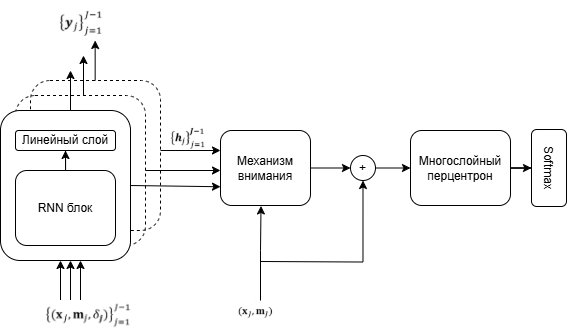
\includegraphics[width=1\textwidth]{../figures/dynamic_deephit_scheme_only_architecture.png}
	\caption{Архитектура модели}
\end{figure}

Наша модель состоит из трех частей:

1. RNN блок - обрабатывает входящую последовательно векторов признаков на разных временных срезах

2. Механизм внимания выделяет ключевую информацию из последовательности

3. Многослойный перцептрон с Softmax агрегирует информацию в вектор вероятностей

Подобная архитектура используется во многих моделях выживаемости и хорошо себя зарекомендовала. Наш результат, таким образом, состоит не в новой архитектуре, а новой функции потерь. Мы далее покажем одно из основных свойств добавки $\mathcal{L}_2$ этой функции потерь.  


\section{Свойства добавки $\mathcal{L}_2$}

Выше мы упомянули, что $\mathcal{L}_2$ обладает ранжирующим свойством с точки зрения C-индекса. Сформулируем строго это утверждение и докажем его для двух вышеописанных постановок задач. Прежде введем понятие отступа, которое аналогично по смыслу понятию отступа в задаче классификации: 

\begin{definition}
Пусть $(i,j)$ - пара абонентов, для которых произошло событие оттока $k$ в моменты времени $\tau^{(i)}$ и $\tau^{(j)}$ соответственно, причем $\tau^{(i)} < \tau^{(j)}$. Тогда в случае постановки с одним вектором-признаком отступ $M_{k,i,j}$ определяется как: 

$$M_{k,i,j} = \hat{F}_k(\tau^{(i)}|\mathbf{x}^{(i)}) - \hat{F}_k(\tau^{(i)}|\mathbf{x}^{(j)}) $$ 

С случае постановки для временного ряда векторов-признаков отступ $M_{k,i,j}$ определяется как:

$$M_{k,i,j} = \hat{F}_k(s^i+t_{J^i}^i|\mathcal{X}^i) - \hat{F}_k(s^i+t_{J^j}^j|\mathcal{X}^j)$$

\end{definition}

В задаче классификации отступ является мерой того, насколько уверенно модель правильно классифицирует объекты. В нашей постановке анализа выживаемости отступ является мерой того, насколько модель уверенно правильно упорядочивает абонентов. Теоремы ниже являются точным выражением того, что добавка $\mathcal{L}_2$ тем ниже, чем выше отступы $M_{k,i,j}$. 

\begin{theorem}
	Пусть $\mathcal{L}_2 =\sum_{k=1}^K\alpha_k\cdot\sum_{i\neq j}A_{k,i,j}\cdot\eta\left(\hat{F}_k(\tau^{(i)}|\mathbf{x}^{(i)}),\hat{F}_k(\tau^{(i)}|\mathbf{x}^{(j)})\right)$ - добавка к функции потерь в смысле постановки с одним вектором-признаком. Тогда $\mathcal{L}_2$ является убывающей от отступов функцией.  
\end{theorem}

\begin{theorem}
	Пусть $\mathcal{L}_2 =\sum_{k=1}^K\alpha_k\cdot\sum_{i\neq j}A_{k,i,j}\cdot\eta\left(\hat{F}_k(s^i+t_{J^i}^i|\mathcal{X}^i) , \hat{F}_k(s^i+t_{J^j}^j|\mathcal{X}^j))\right)$ - добавка к функции потерь в смысле постановки для временного ряда векторов-признаков. Тогда $\mathcal{L}_2$ является убывающей от отступов функцией.  
\end{theorem}

\begin{proof}
	В обеих постановках добавка принимает вид: 
	
	$$\mathcal{L}_2 =\sum_{k=1}^K\alpha_k\cdot\sum_{i\neq j}A_{k,i,j}\cdot\exp\left(-\frac{M_{k,i,j}}{\sigma}\right)$$
	
	поэтому выражения для производных принимают вид: 
	
	$$ 
	\frac{\partial \mathcal{L}_2}{\partial M_{k,i,j}} = 
	-\frac{1}{\sigma} \sum_{k=1}^K\alpha_k\cdot A_{k,i,j}\cdot\exp\left(-\frac{M_{k,i,j}}{\sigma}\right) < 0
	 $$
	
	откуда следуют утверждения теорем.
\end{proof}


Таким образом, смысл добавки $\mathcal{L}_2$ сводится к штрафованию модели появлению маленьких отступов, которые связаны с нарушением верной упорядоченности абонентов и понижением C-индекса. 


\chapter{Численные эксперименты}

\section{Описание постановки задачи}

В численных экспериментах рассматривался частный случай общей поставноки задачи при котором $K = 1$ - события оттока не различаются между собой. При этом производительность моделей сравнивалась на задачах бинарной и многоклассовой классификации: 

1. В задаче бинарной классификации предсказываются вероятности двух классов - сохранение абонента в следующий месяц (таргет $q = 0$) и отток абонента в следующий месяц (таргет $q = 1$)

2. В задаче многоклассовой классификации предсказываются вероятности следующих четырех классов: отток в конец текущего месяца (таргет $q = 0$), отток в конец следующего месяца (таргет $q = 1$), отток в конец послеследующего месяца (таргет $q = 3$) и сохранение абонента на конец послеследующего месяца (таргет $q = 4$). Новые признаки, генерируемые моделью, представляют собой вектор $(x_0,x_1,x_2,x_3,x_4) \in \mathbb{R}^{5}$, где $x_i$ - вероятность выживания в $i$-ый месяц, где за $0$ месяц берется июнь 2024




\section{Описание данных}

Эксперименты проводились на данных компании Мегафон, собранных с начала апреля 2024 до конца октября 2024. 

Обучающая выборка состоит из 2.7 миллионов примеров, валидационная и тестовая выборки содержат по 600 и 800 тыс. обучающих примеров соответственно. 

Для модели DeepHit обучающая выборка предварительно была нормирована. Для CatBoost нормировка не проводилась. Для подбора гиперпараметров CatBoost была использована библиотека optuna. Для архитектуры DeepHit был использован многослойный перцептрон.

\section{Критерии качества}

Для анализа качества была использована функция reports из модуля scoring, которая строит отчеты-таблицы по моделям. Отчет-таблица демонстирует, насколько хорошо модель отделяет каждый из классов от всех остальных (One-vs-All подход). Опишем структуру этого отчета. Для начала введем понятие топ перцентиля: 

\begin{definition}
Топ-$p$ перцентиль для некоторого класса $q$ определяется как квантиль уровня $1-p$ для предсказанных моделью вероятностей класса $q$.
\end{definition}

В рамках One-vs-All подхода, по определению будем считать, что если предсказанная моделью вероятность класса $q$ больше порога в топ-$p$ перцентиль для некоторого заранее фиксированного $p$, то ответом модели будет класс $q$, иначе ответом будут все классы, кроме $q$.

В случае задачи бинарной классификации рассматриваются только топ перцентили для класса $q = 1$, соответствующему оттоку абонента, а в случае многоклассовой классификации - топ-перцентили для всех классов. При этом в многоклассовой постановке каждому классу соответствует свой отчет, показывающий, как хорошо данный класс отделяется от всех остальных. 

Стоблцы таблицы соответствуют широко распространенным метрикам классификации - Precision, Recall, F1 и AUC. Строки таблицы соответствуют различным топ-$p$ перцентилям для данного класса. Таким образом можно сравнивать метрики в зависимости от различных порогов вероятностей. 

\section{Метод подбора гиперпараметров и шага обучения}

\subsection{Grid Search}

Для подбора гиперпараметров использовался известный метод Grid Search. Его сущность заключается в следующем: 

1. Определение сетки гиперпараметров: для каждого гиперпараметра задаются конкретные значения или диапазон значений. 

2. Перебор всех комбинаций:алгоритм последовательно проверяет каждую возможную комбинацию гиперпараметров, создавая новую модель для каждой комбинации и оценивая её качество на заранее выбранном метричном показателе.

3. Оценка качества моделей: качество каждой модели оценивается на отдельной тестовой выборке.

4. Выбор лучшей комбинации: после проверки всех комбинаций выбирается та комбинация гиперпараметров, которая дала наилучшее значение целевой метрики качества. 

\subsection{Learning Rate Finder}

Процедура Learning Rate Finder позволяет найти оптимальное значение шага обучения. Она работает следующим образом: 

1. Выбор начальных и конечных границ: выбирается интервал скоростей обучения, в пределах которого будет проводиться исследование. Скорость обучения изменяется экспоненциально между начальной и конечной точкой. Это значит, что каждое следующее значение увеличивается по отношению к предыдущему на постоянный коэффициент. 

2. Быстрое обучение и сбор статистики: модель быстро обучается на небольшом числе эпох или батчей, используя различные значения скорости обучения, вычисляемые на каждом шаге согласно формуле выше. На каждом этапе фиксируются потери модели.

3. Анализ результатов: полученная зависимость потерь от скорости обучения визуально отображается графиком. Оптимальной скоростью обучения считается точка, где потеря резко снижается, но ещё не начала увеличиваться снова. Этот момент соответствует точке максимальной эффективности градиентного спуска.



\section{DeepHit в задаче бинарной классификации}



\subsection{Число эпох обучения = 3}

Для начала было использовано три эпохи обучения. График функции потерь имеет вид:

\begin{figure}[H]
	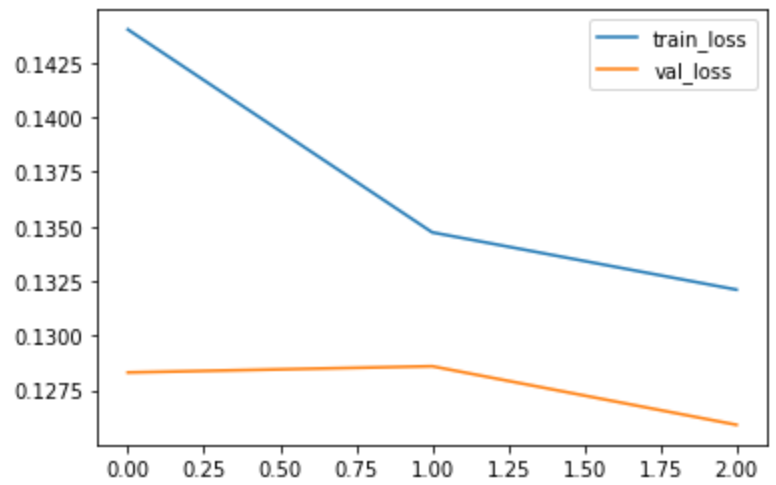
\includegraphics[width=0.45\textwidth]{../figures/deephit_losses_3_epoch.png}
	\caption{Функция потерь}
\end{figure}

Ниже поедставлено сравнение метрик на ТОП 10\% для DeepHit и CatBoost. 

\begin{figure}[H]
	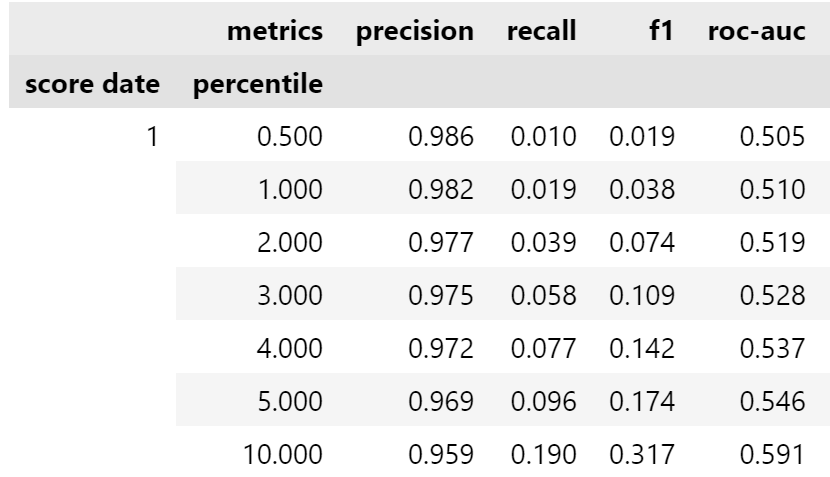
\includegraphics[width=0.45\textwidth]{../figures/deephit_reports_3_epoch.png}
	\caption{Результаты DeepHit}
	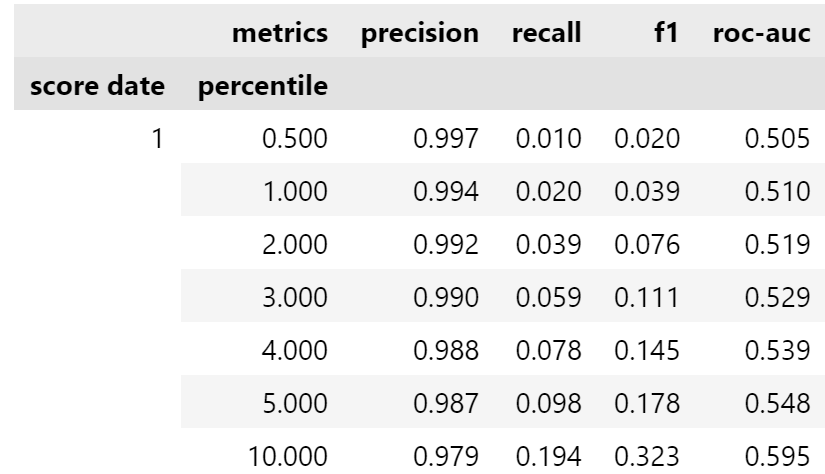
\includegraphics[width=0.45\textwidth]{../figures/catboost_reports.png}
	\caption{Результаты CatBoost}
\end{figure}

\subsection{Число эпох обучения = 30}

На этом этапе мы заметно увеличили число эпох обучения DeepHit. Такое число эпох оказалось оптимальным - исследования показали, что после 30 эпох происходит переобучение и функция потерь на валидационной выборке начинает вести себя нестабильно. Поэтому было принято решение установить число эпох не более 30.  


\section{DeepHit в задаче многоклассовой классификации}

\begin{figure}[H]
	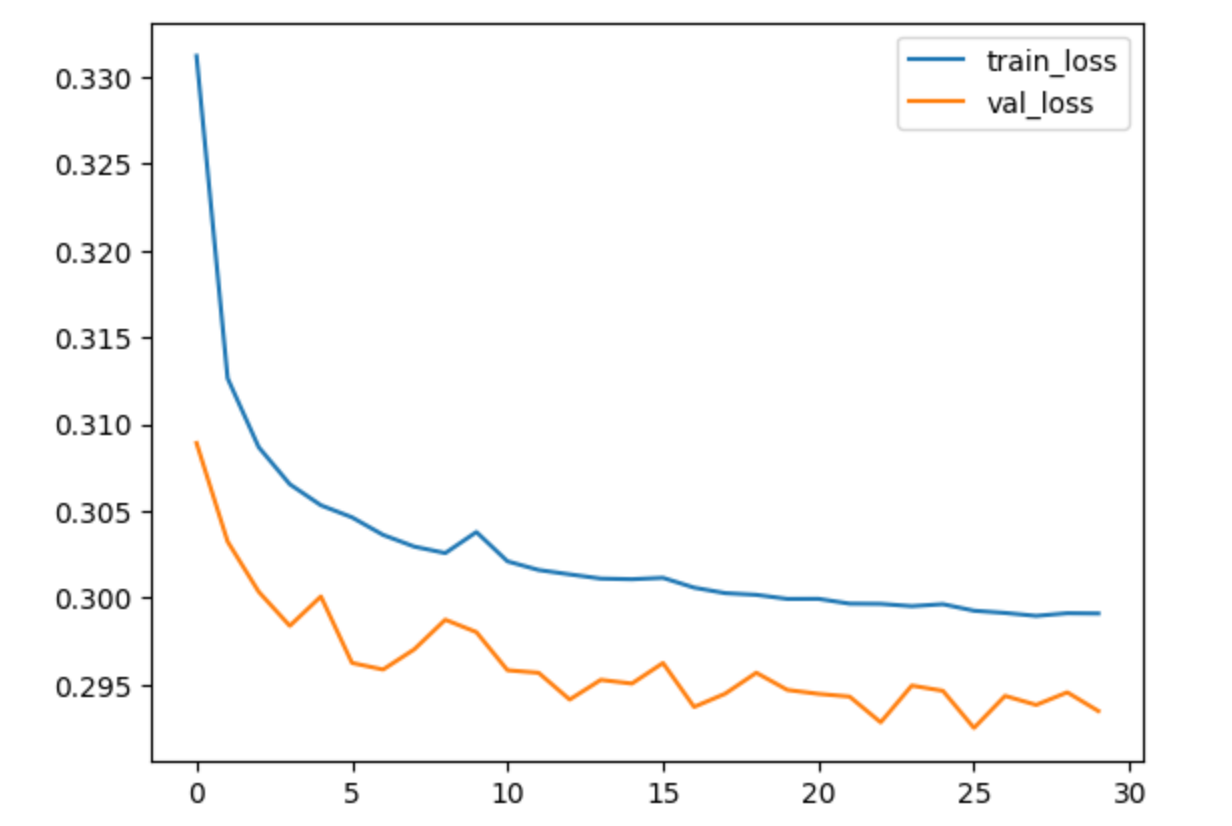
\includegraphics[width=\textwidth]{../figures/deephit_losses_30_epoch.png}
	\caption{Функция потерь для модели DeepHit}
\end{figure}

\begin{figure}[H]
	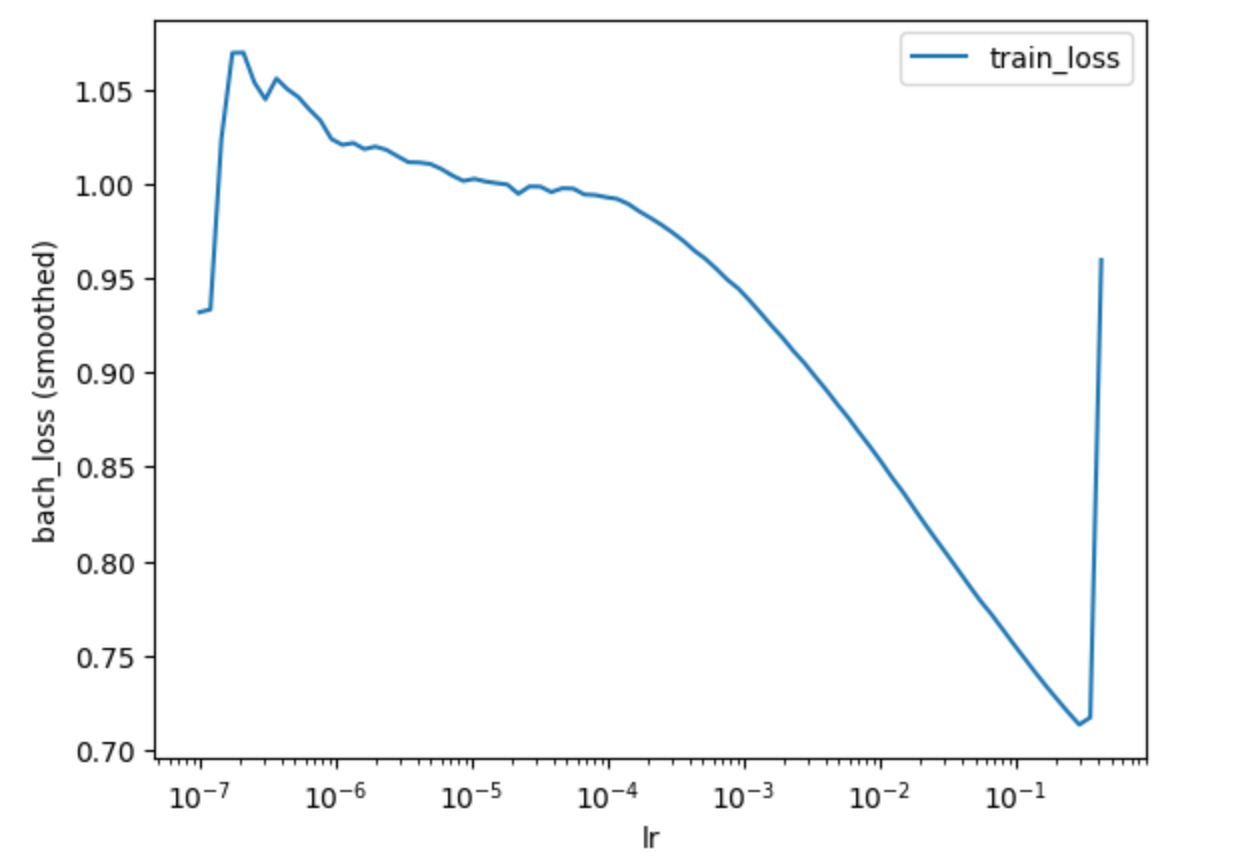
\includegraphics[width=\textwidth]{../figures/deephit_losses_30_epoch_lr.png}
	\caption{Выбор оптимального шага обучения для модели DeepHit}
\end{figure}

\subsection{Вклад признаков моделей}

Точность на исходных 50 признаках: $73.1\%$

Точность на 5 признаках модели: $80.6\%$

Потеря в точности: $7.5\%$


\subsection{Значение C-индекса модели}

Значение C индекса: $0.74$

\subsection{Интерпретация вероятностей выживания}

Ниже приведены вероятности выживания данной модели для разных месяцев: 

\begin{figure}[H]
	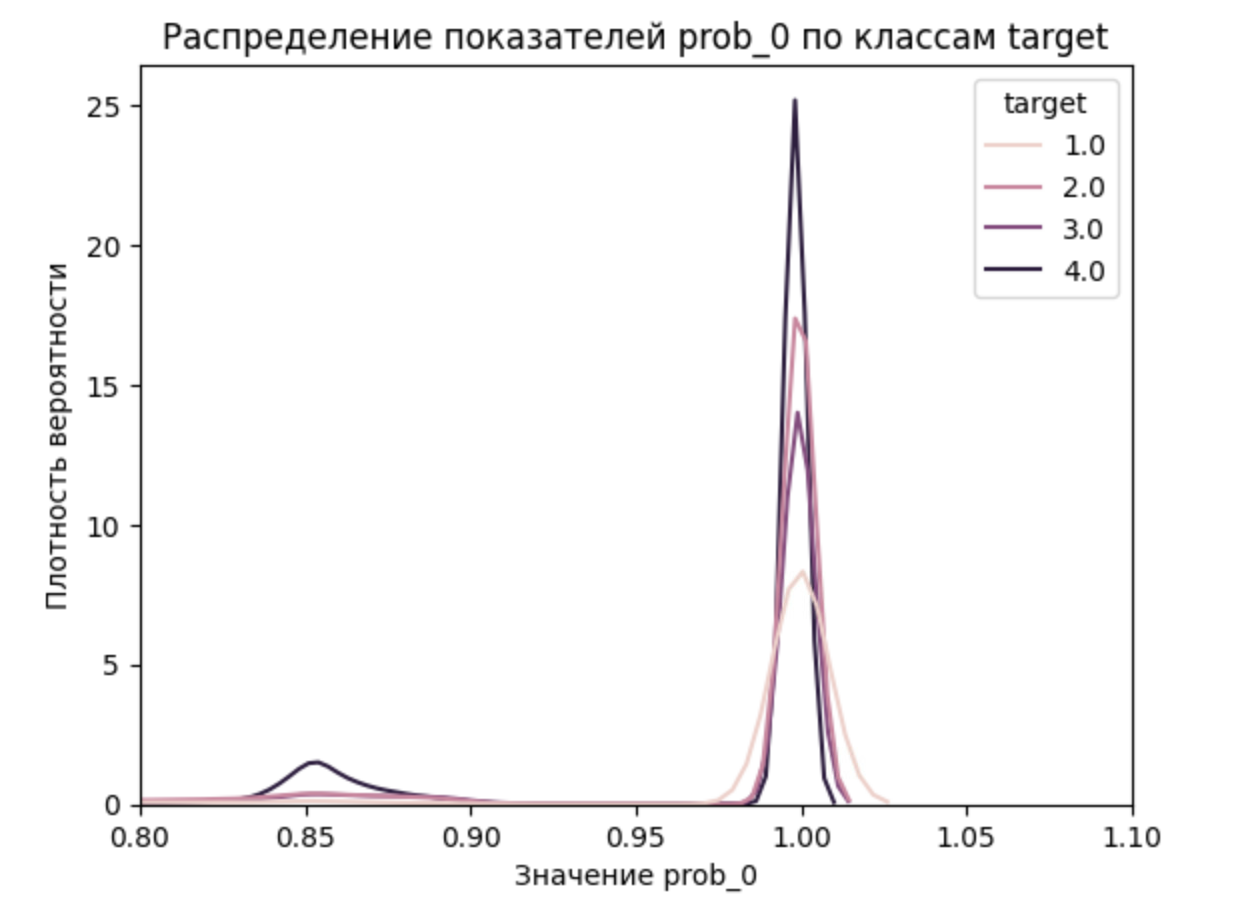
\includegraphics[width=0.9\textwidth]{../figures/prob_0_deephit.png}
	\caption{Вероятность выживания в июнь 2024 для модели DeepHit}
\end{figure}

\begin{figure}[H]
	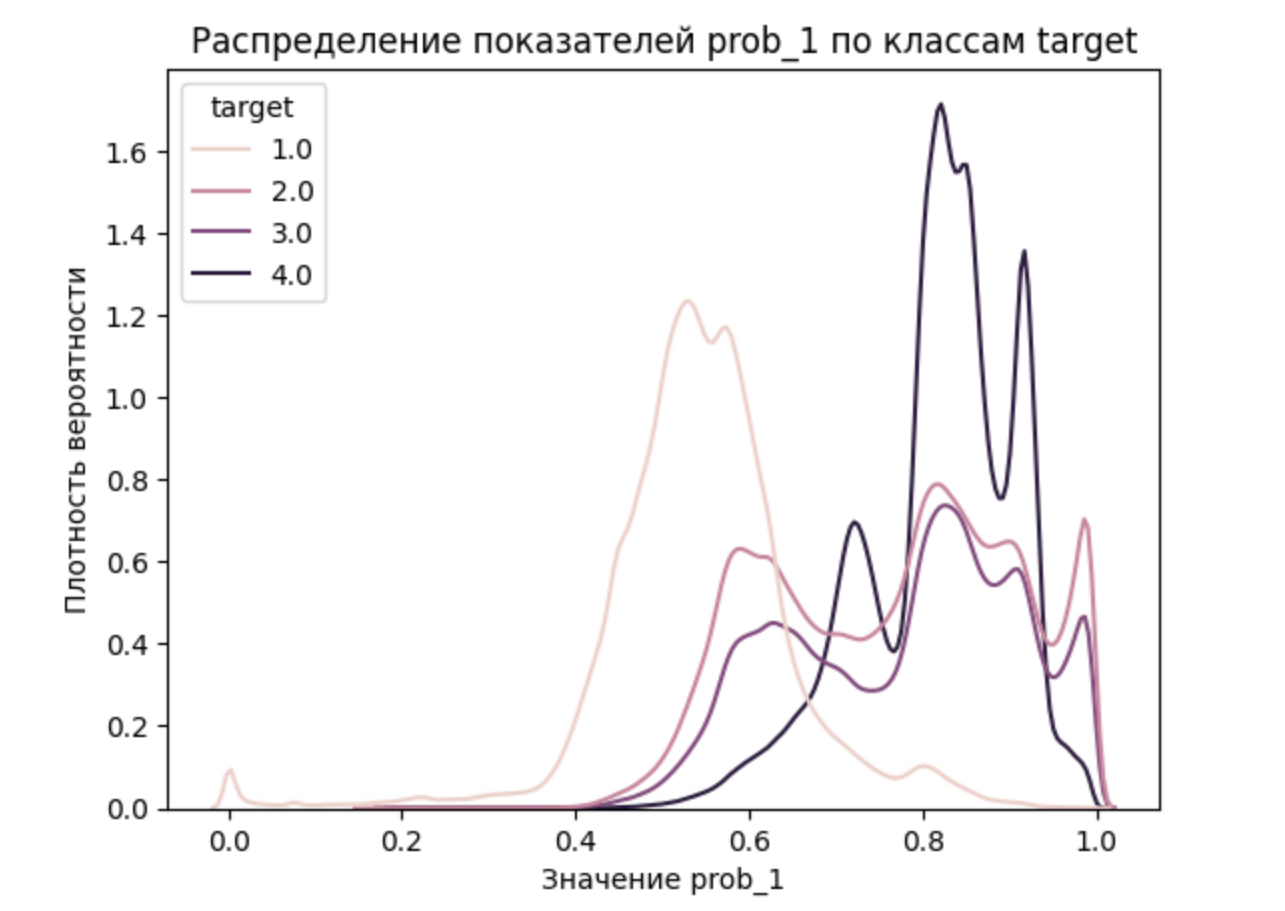
\includegraphics[width=0.9\textwidth]{../figures/prob_1_deephit.png}
	\caption{Вероятность выживания в июль 2024 для модели DeepHit}
\end{figure}

\begin{figure}[H]
	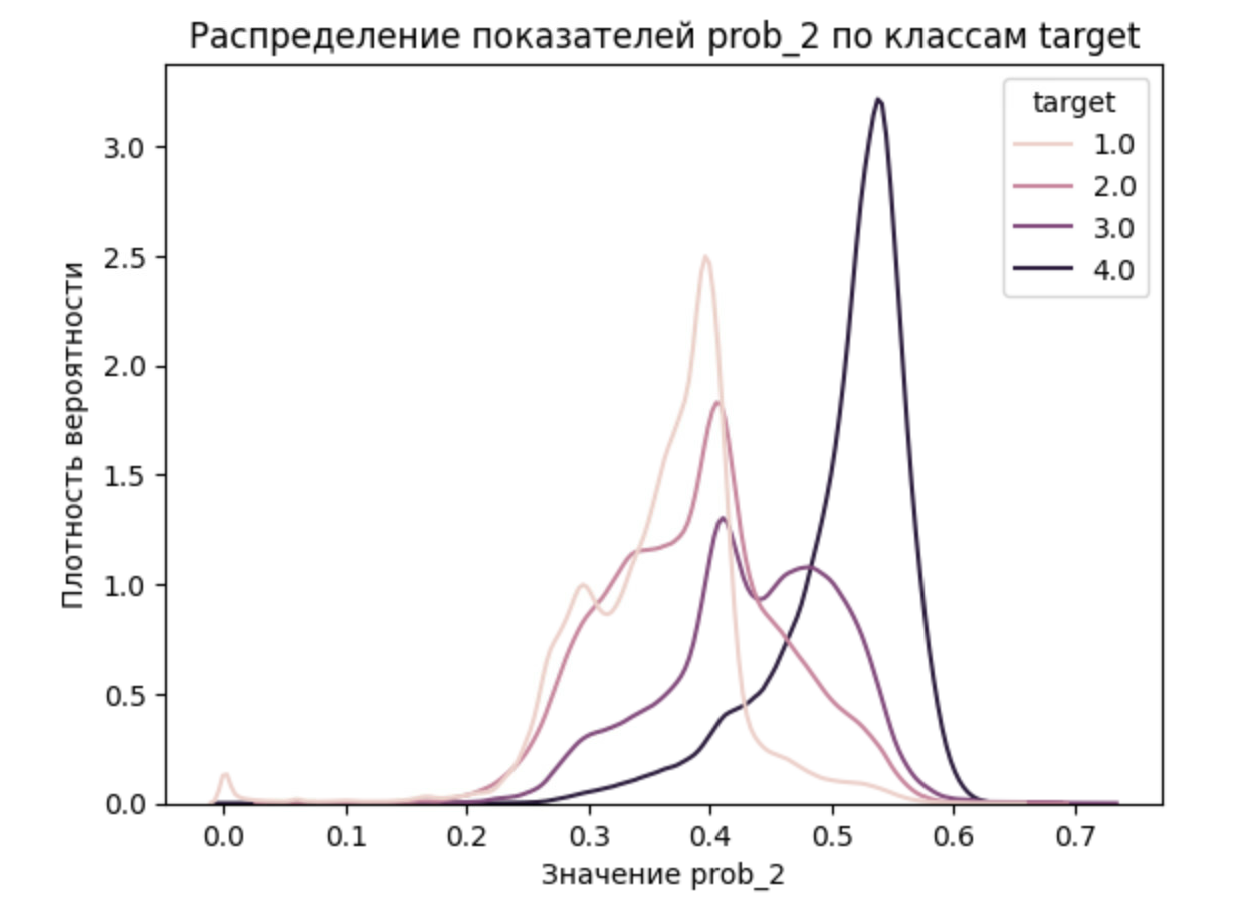
\includegraphics[width=0.9\textwidth]{../figures/prob_2_deephit.png}
	\caption{Вероятность выживания в август 2024 для модели DeepHit}
\end{figure}

\begin{figure}[H]
	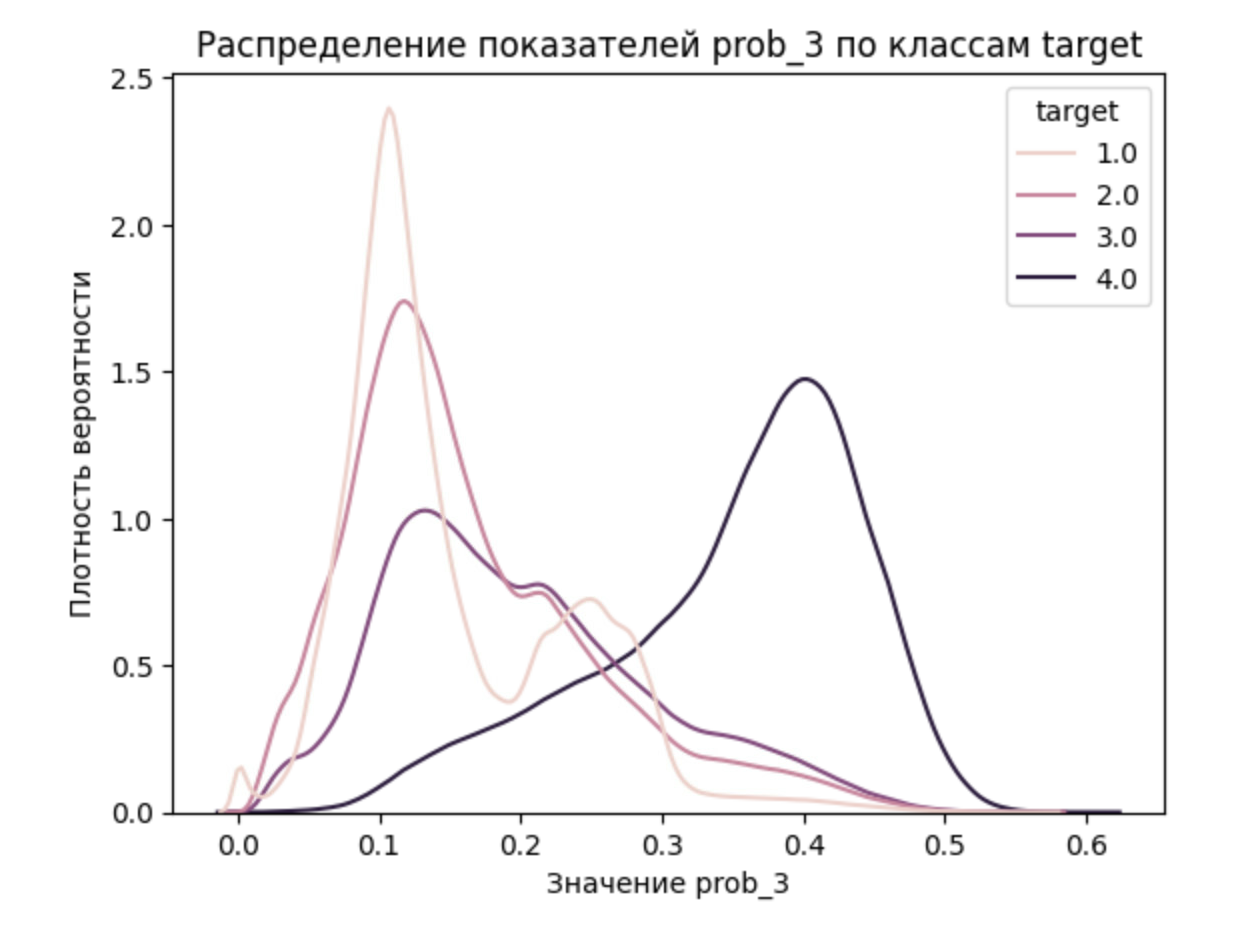
\includegraphics[width=0.9\textwidth]{../figures/prob_3_deephit.png}
	\caption{Вероятность выживания в сентябрь 2024 для модели DeepHit}
\end{figure}

Видим логичную закономерность: чем более поздний месяц мы рассматриваем, тем ниже будет вероятность. 

Видно, что модель хорошо отделяет таргет 4 (абоненты, которые не оттекли) от оттекших абонентов (таргеты 1, 2 и 3), однако плохо отличает оттекших абонентов между собой. 

\section{PMF в задаче многоклассовой классификации}

Ниже приведены вероятности выживания данной модели для разных месяцев: 

\begin{figure}[H]
	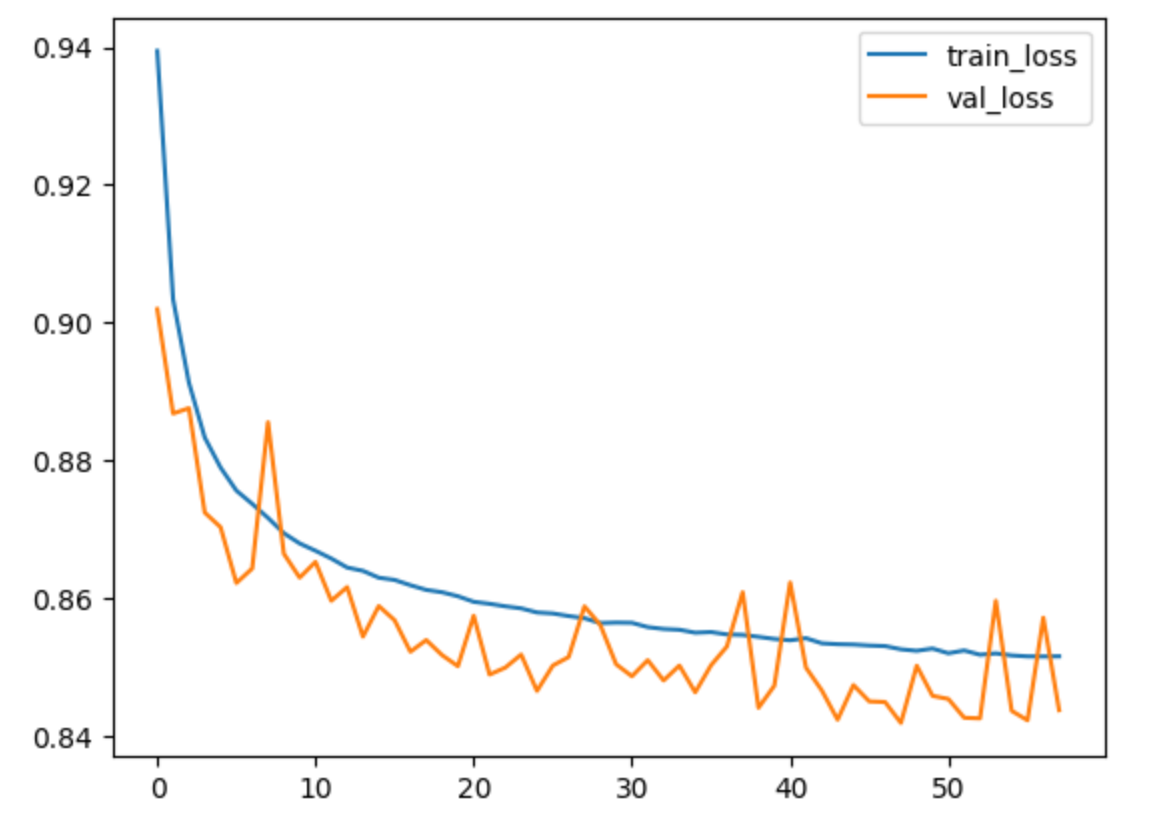
\includegraphics[width=\textwidth]{../figures/pmf_losses_30_epoch.png}
	\caption{Функция потерь для модели PMF}
\end{figure}

\begin{figure}[H]
	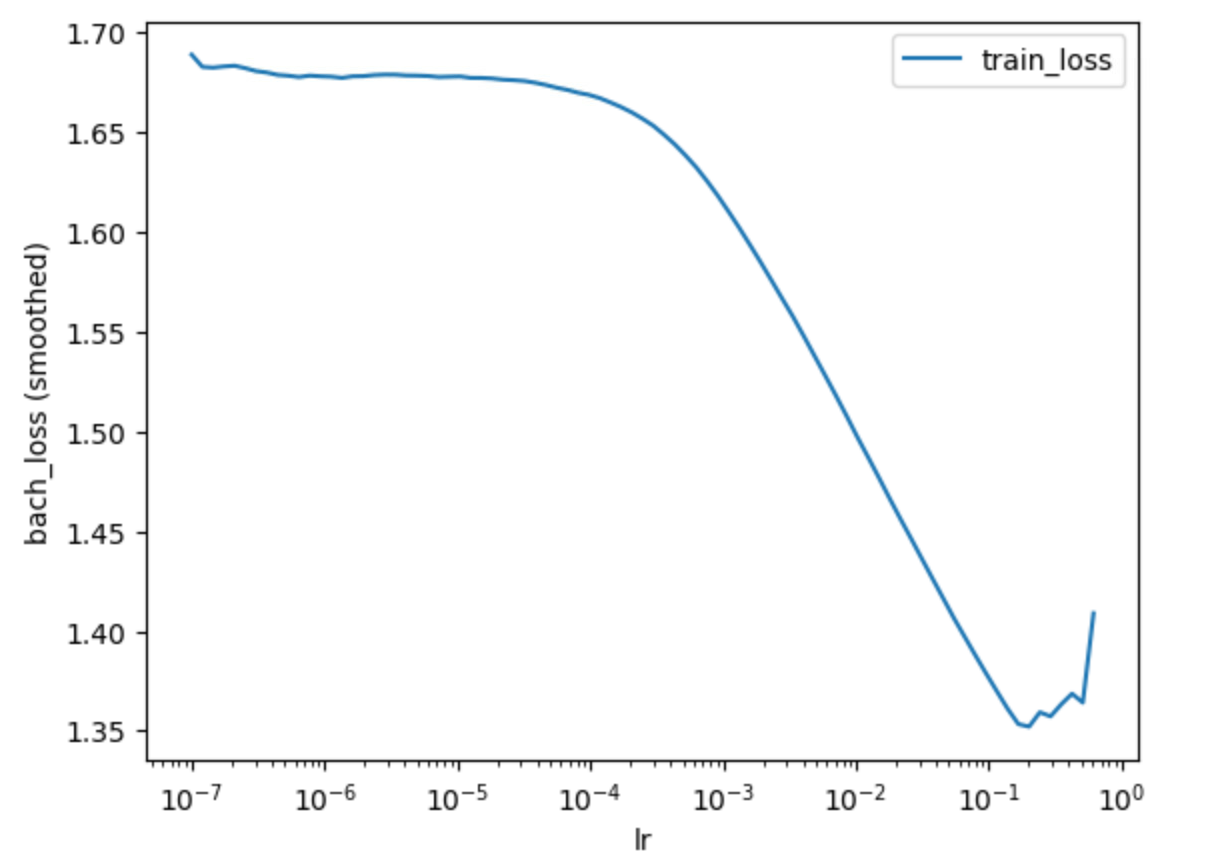
\includegraphics[width=\textwidth]{../figures/pmf_losses_30_epoch_lr.png}
	\caption{Выбор оптимального шага обучения для модели PMF}
\end{figure}

\subsection{Вклад признаков моделей}

Точность на исходных 50 признаках: $75.2\%$

Точность на 5 признаках модели: $80.6\%$

Потеря в точности: $5.4\%$

\subsection{Значение C-индекса модели}

Значение C индекса: $0.75$

\subsection{Интерпретация вероятностей выживания}

Ниже приведены вероятности выживания данной модели для разных месяцев: 

\begin{figure}[H]
	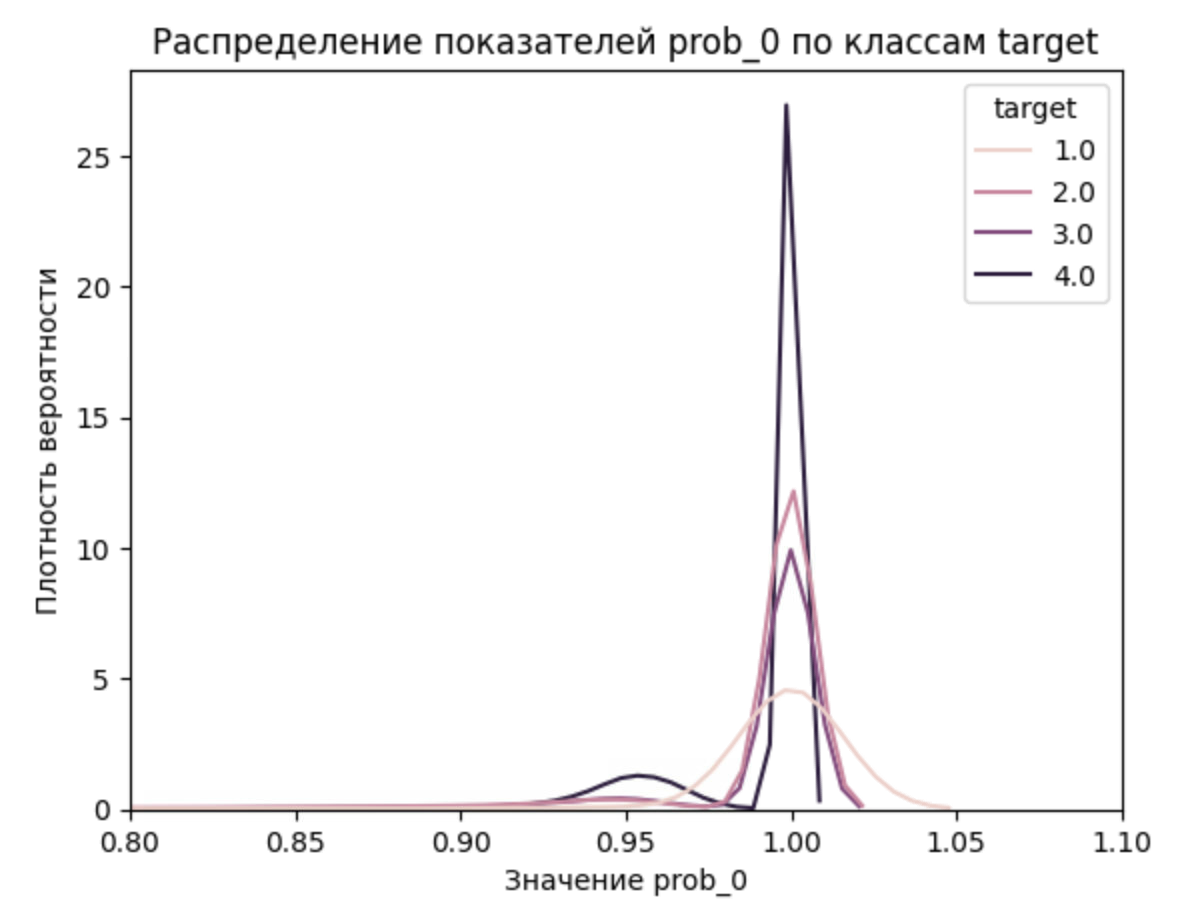
\includegraphics[width=0.9\textwidth]{../figures/prob_0_pmf.png}
	\caption{Вероятность выживания в июнь 2024 для модели PMF}
\end{figure}

\begin{figure}[H]
	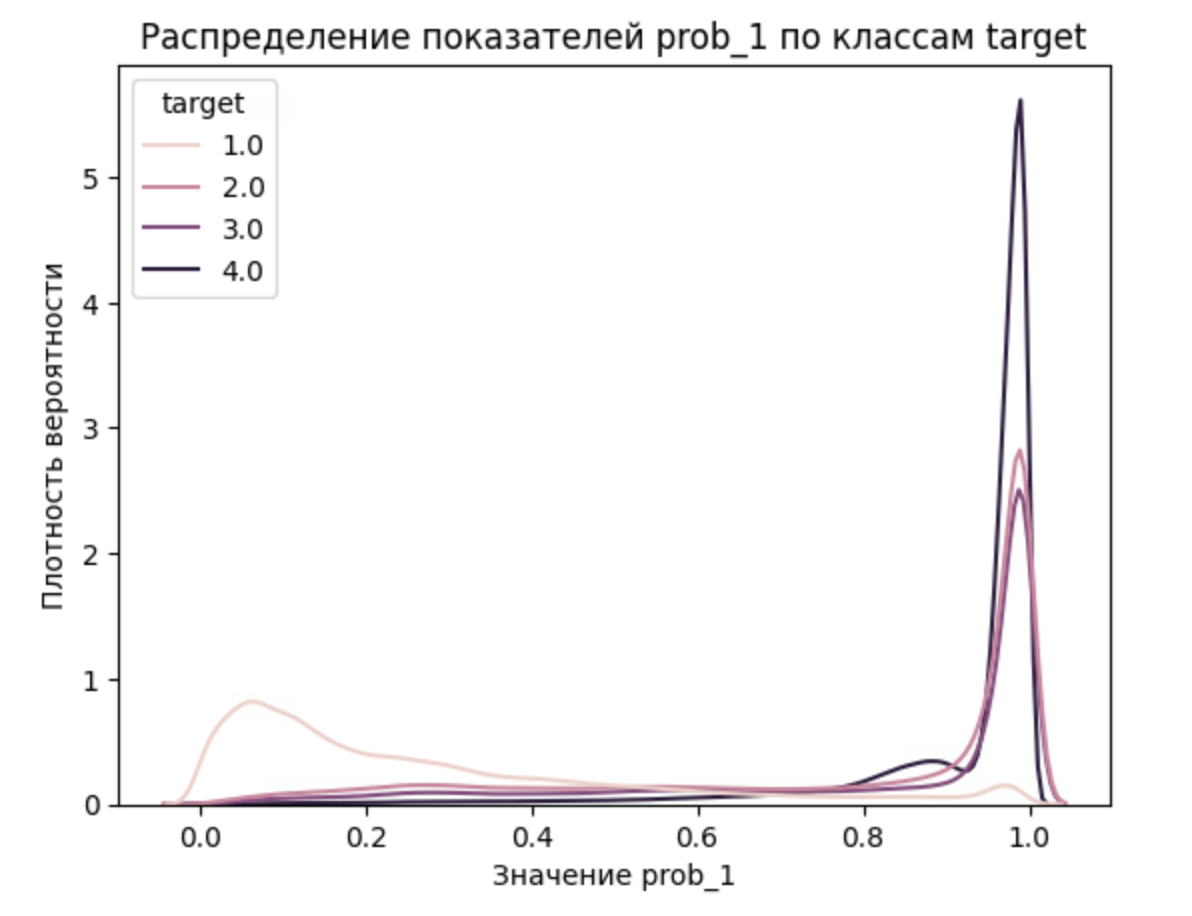
\includegraphics[width=0.9\textwidth]{../figures/prob_1_pmf.png}
	\caption{Вероятность выживания в июль 2024 для модели PMF}
\end{figure}

\begin{figure}[H]
	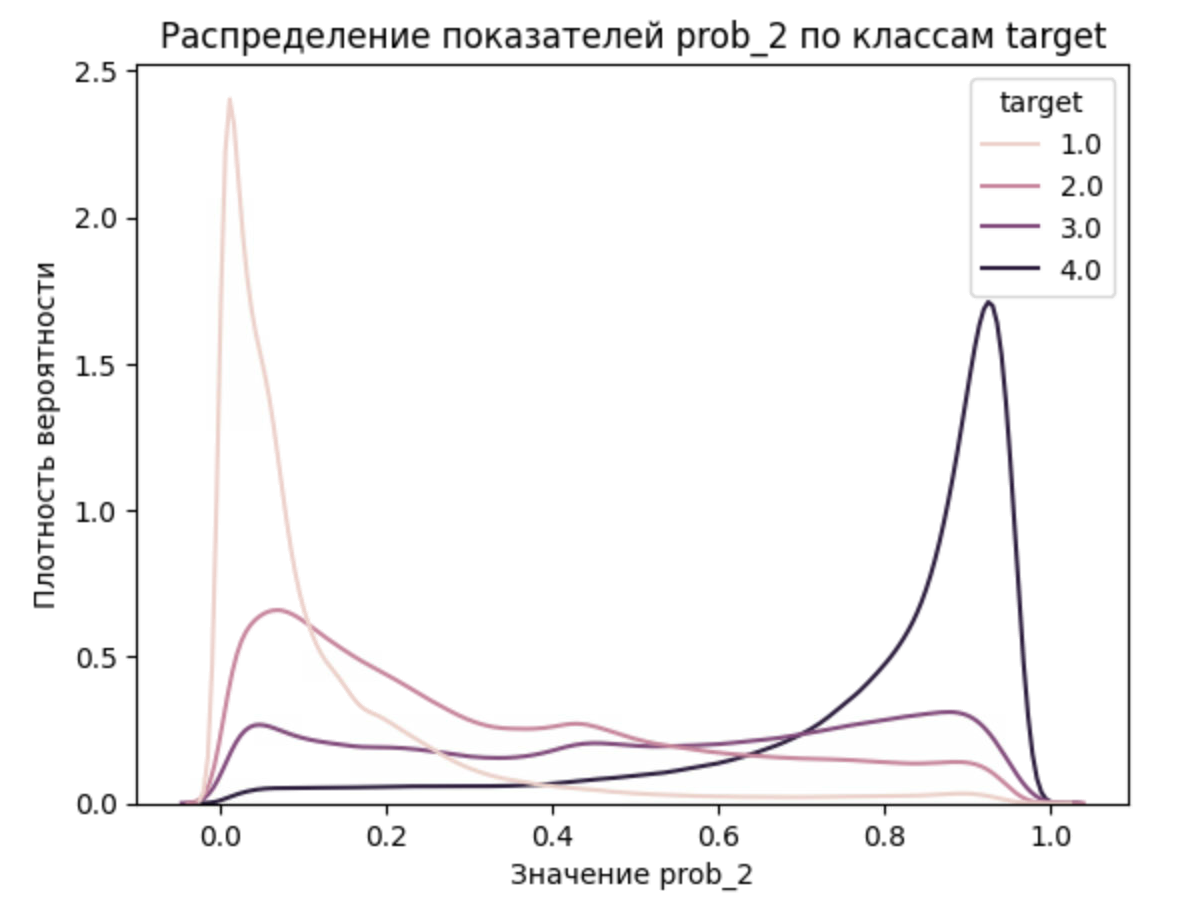
\includegraphics[width=0.9\textwidth]{../figures/prob_2_pmf.png}
	\caption{Вероятность выживания в август 2024 для модели PMF}
\end{figure}

\begin{figure}[H]
	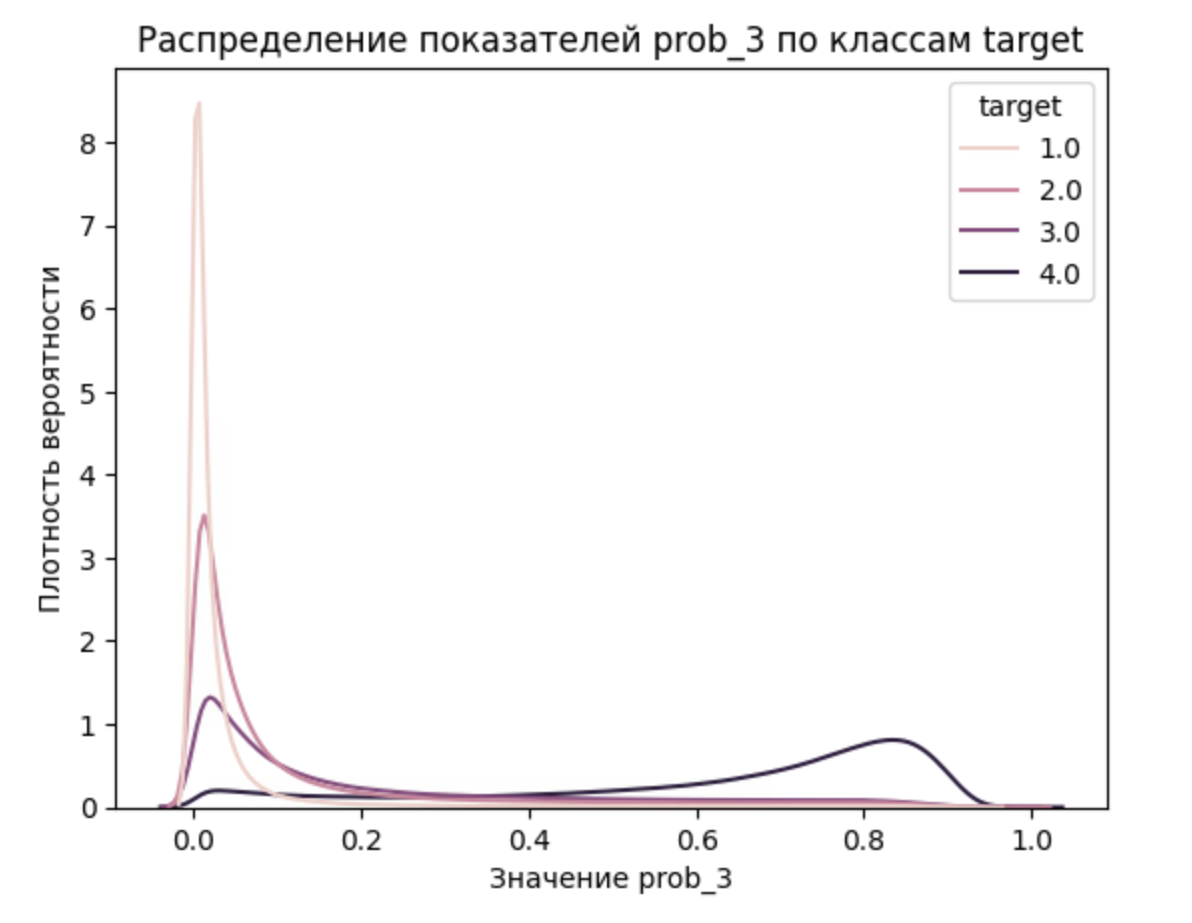
\includegraphics[width=0.9\textwidth]{../figures/prob_3_pmf.png}
	\caption{Вероятность выживания в сентябрь 2024 для модели PMF}
\end{figure}

Модель хорошо отделяет таргет 4 (абоненты, которые не оттекли) от оттекших абонентов (таргеты 1, 2 и 3), однако плохо отличает оттекших абонентов между собой. 

\section{Nnet-survival в задаче многоклассовой классификации}

Ниже приведены вероятности выживания данной модели для разных месяцев: 

\begin{figure}[H]
	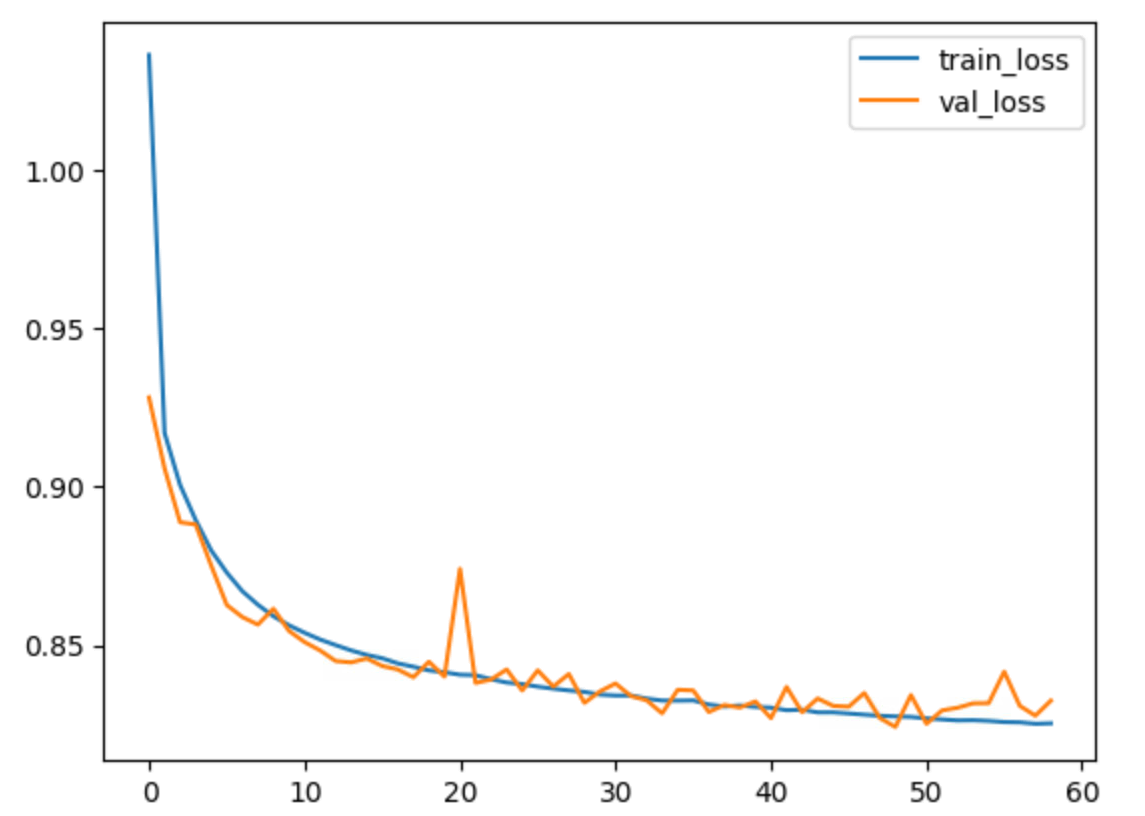
\includegraphics[width=\textwidth]{../figures/nnet_losses_30_epoch.png}
	\caption{Функция потерь для модели Nnet-survival}
\end{figure}

\begin{figure}[H]
	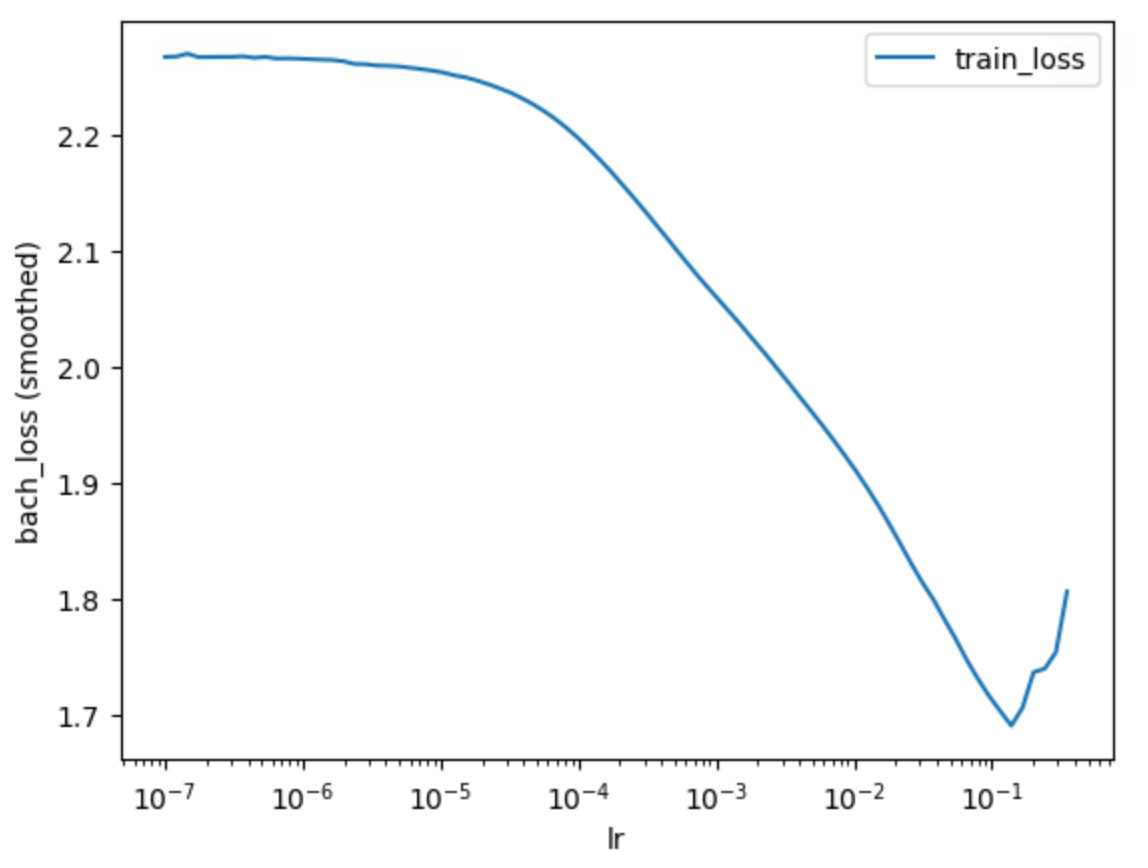
\includegraphics[width=\textwidth]{../figures/nnet_losses_30_epoch_lr.png}
	\caption{Выбор оптимального шага обучения для модели Nnet-survival}
\end{figure}

\subsection{Вклад признаков моделей}

Точность на исходных 50 признаках: $74.8\%$

Точность на 5 признаках модели: $80.6\%$

Потеря в точности: $5.8\%$

\subsection{Значение C-индекса модели}

Значение C индекса: $0.77$

\subsection{Интерпретация вероятностей выживания}

Ниже приведены вероятности выживания данной модели для разных месяцев: 

\begin{figure}[H]
	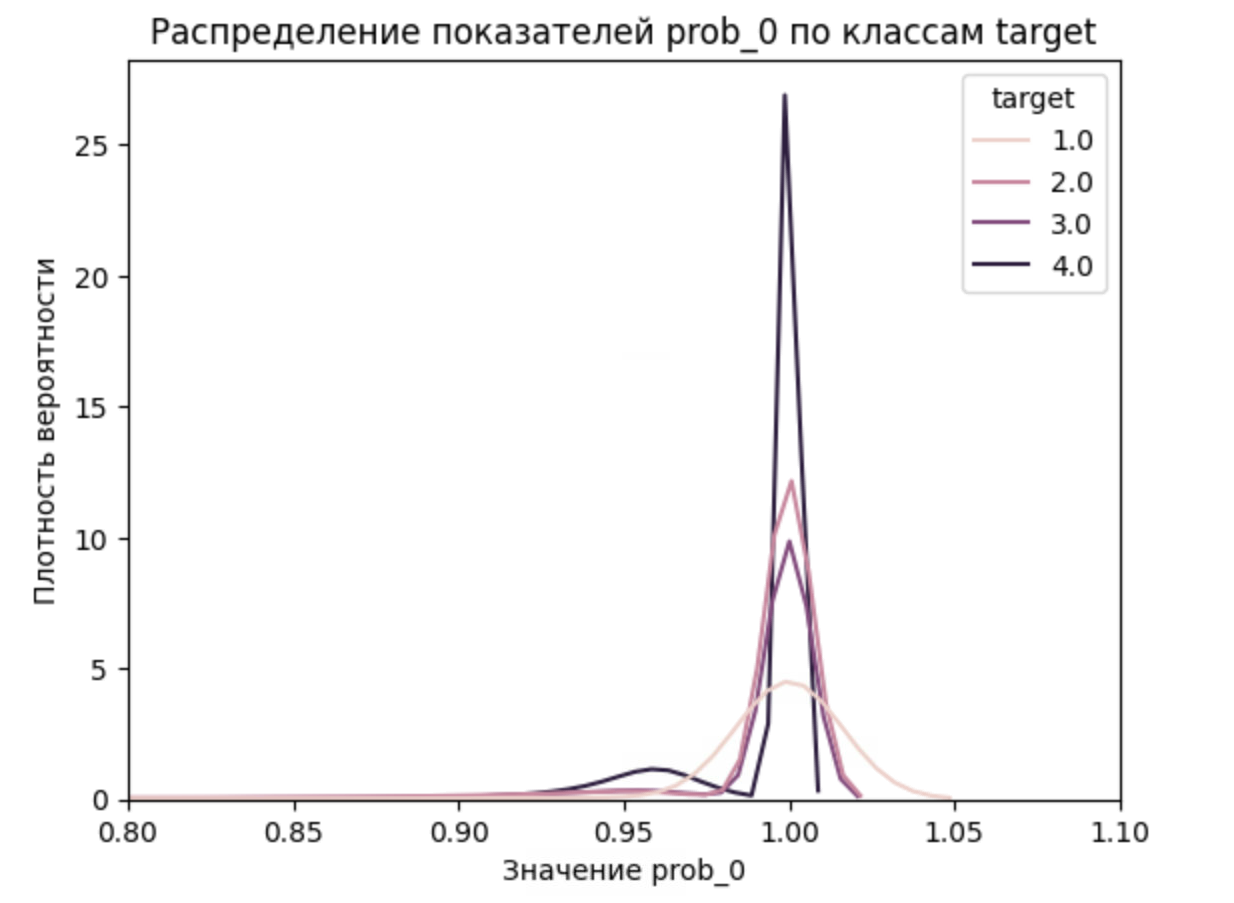
\includegraphics[width=0.9\textwidth]{../figures/prob_0_nnet.png}
	\caption{Вероятность выживания в июнь 2024 для модели Nnet-survival}
\end{figure}

\begin{figure}[H]
	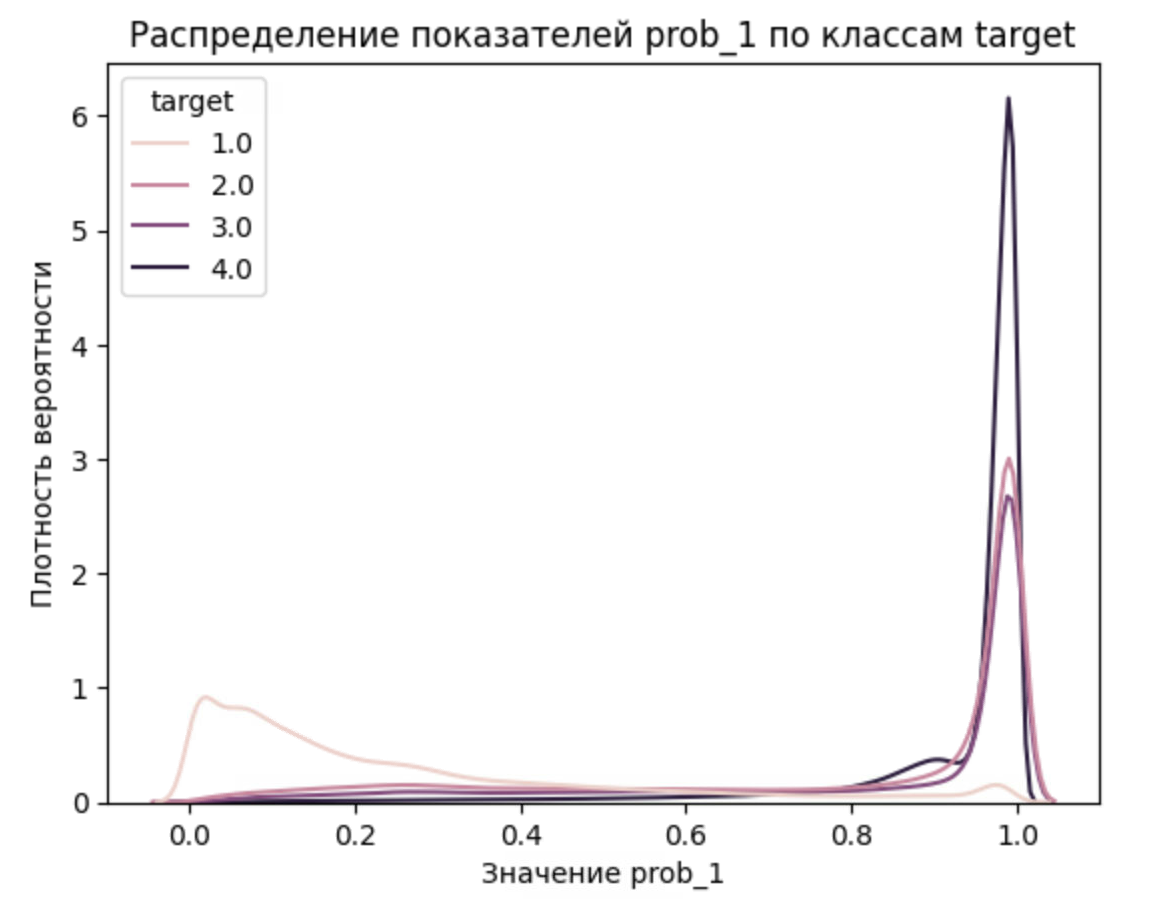
\includegraphics[width=0.9\textwidth]{../figures/prob_1_nnet.png}
	\caption{Вероятность выживания в июль 2024 для модели Nnet-survival}
\end{figure}

\begin{figure}[H]
	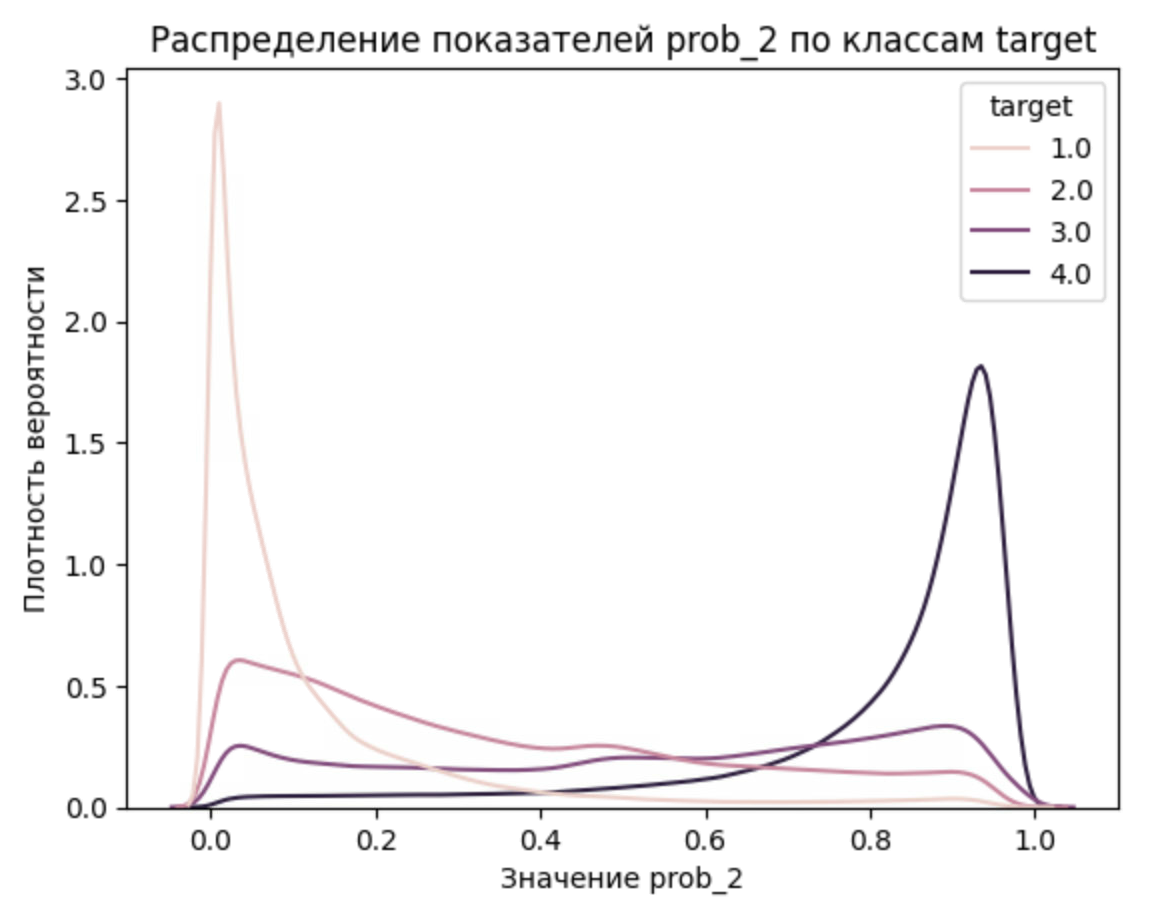
\includegraphics[width=0.9\textwidth]{../figures/prob_2_nnet.png}
	\caption{Вероятность выживания в август 2024 для модели Nnet-survival}
\end{figure}

\begin{figure}[H]
	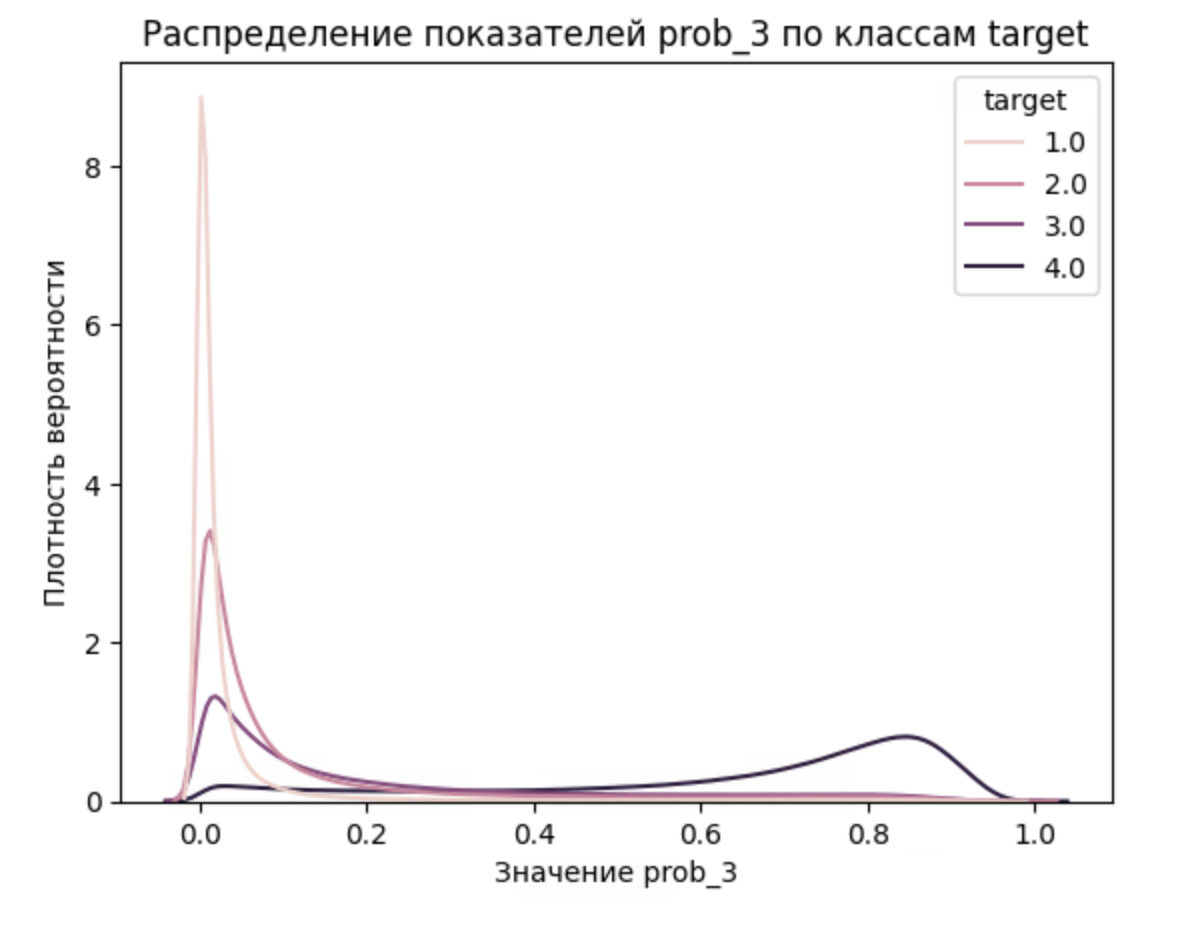
\includegraphics[width=0.9\textwidth]{../figures/prob_3_nnet.png}
	\caption{Вероятность выживания в сентябрь 2024 для модели Nnet-survival}
\end{figure}

Модель хорошо отделяет таргет 4 (абоненты, которые не оттекли) от оттекших абонентов (таргеты 1, 2 и 3), однако плохо отличает оттекших абонентов между собой. 

\section{Наша модель в задаче многоклассовой классификации}

\begin{figure}[H]
	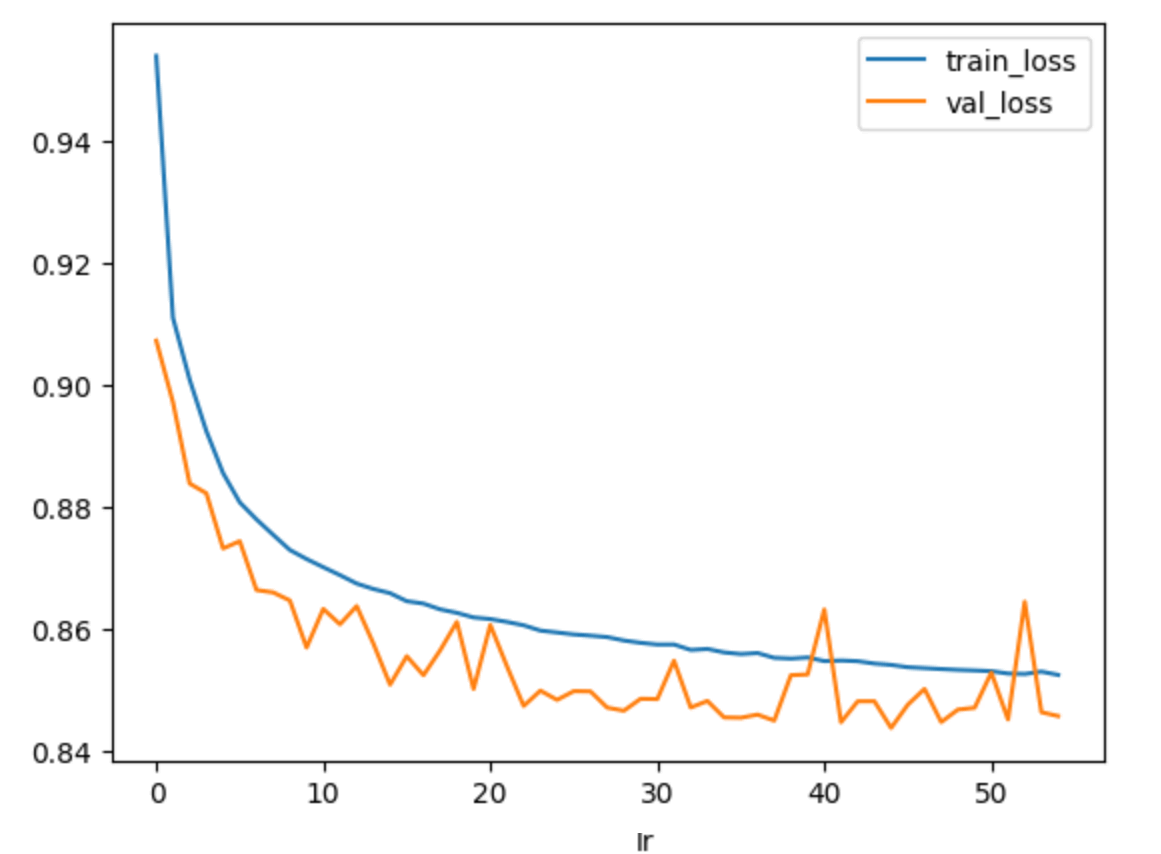
\includegraphics[width=\textwidth]{../figures/our_losses_30_epoch.png}
	\caption{Функция потерь для нашей модели}
\end{figure}

\begin{figure}[H]
	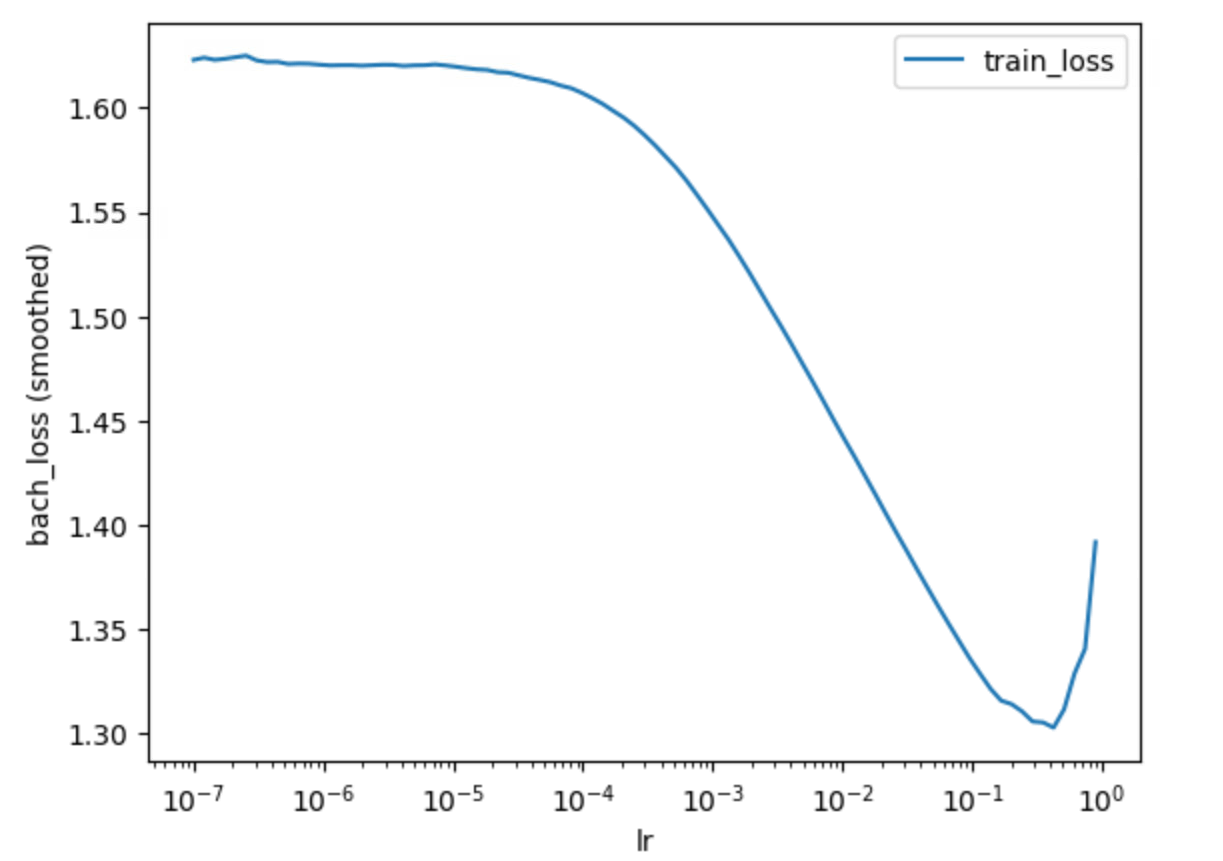
\includegraphics[width=\textwidth]{../figures/our_losses_30_epoch_lr.png}
	\caption{Выбор оптимального шага обучения для нашей модели}
\end{figure}

\subsection{Вклад признаков моделей}

Точность на исходных 50 признаках: $78.5\%$

Точность на 5 признаках модели: $80.6\%$

Потеря в точности: $2.1\%$

\subsection{Значение C-индекса модели}

Значение C индекса: $0.81$

\subsection{Интерпретация вероятностей выживания}

Ниже приведены вероятности выживания данной модели для разных месяцев: 

\begin{figure}[H]
	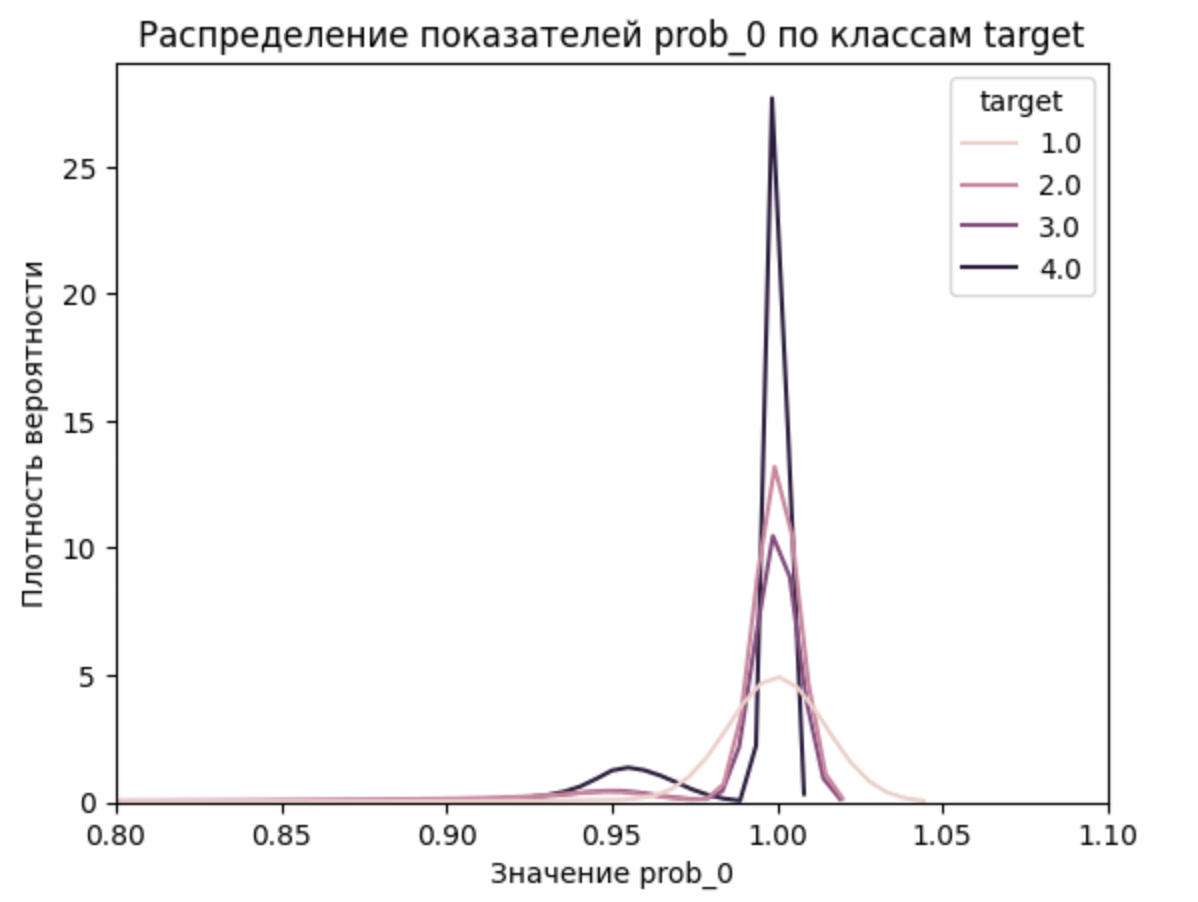
\includegraphics[width=0.9\textwidth]{../figures/prob_0_our.png}
	\caption{Вероятность выживания в июнь 2024 для нашей модели}
\end{figure}

\begin{figure}[H]
	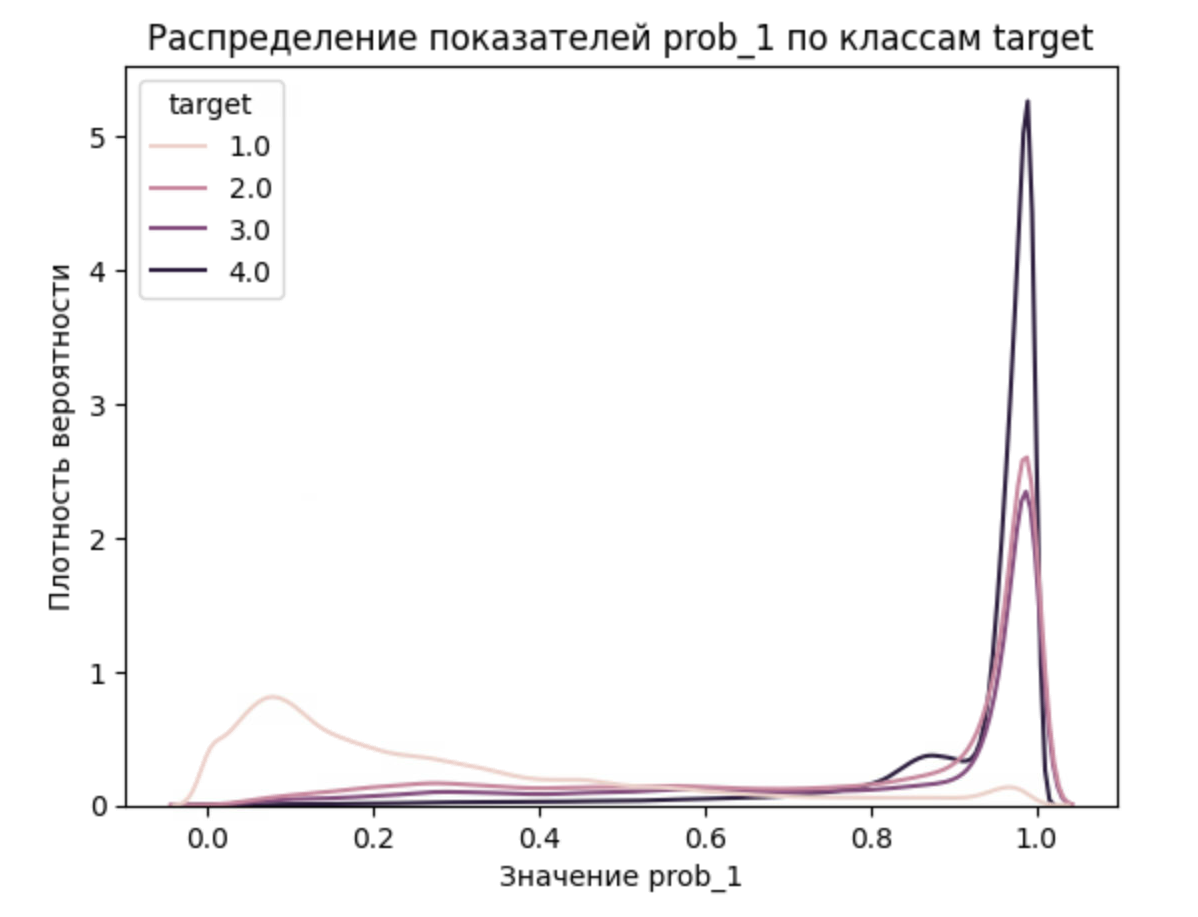
\includegraphics[width=0.9\textwidth]{../figures/prob_1_our.png}
	\caption{Вероятность выживания в июль 2024 для нашей модели}
\end{figure}

\begin{figure}[H]
	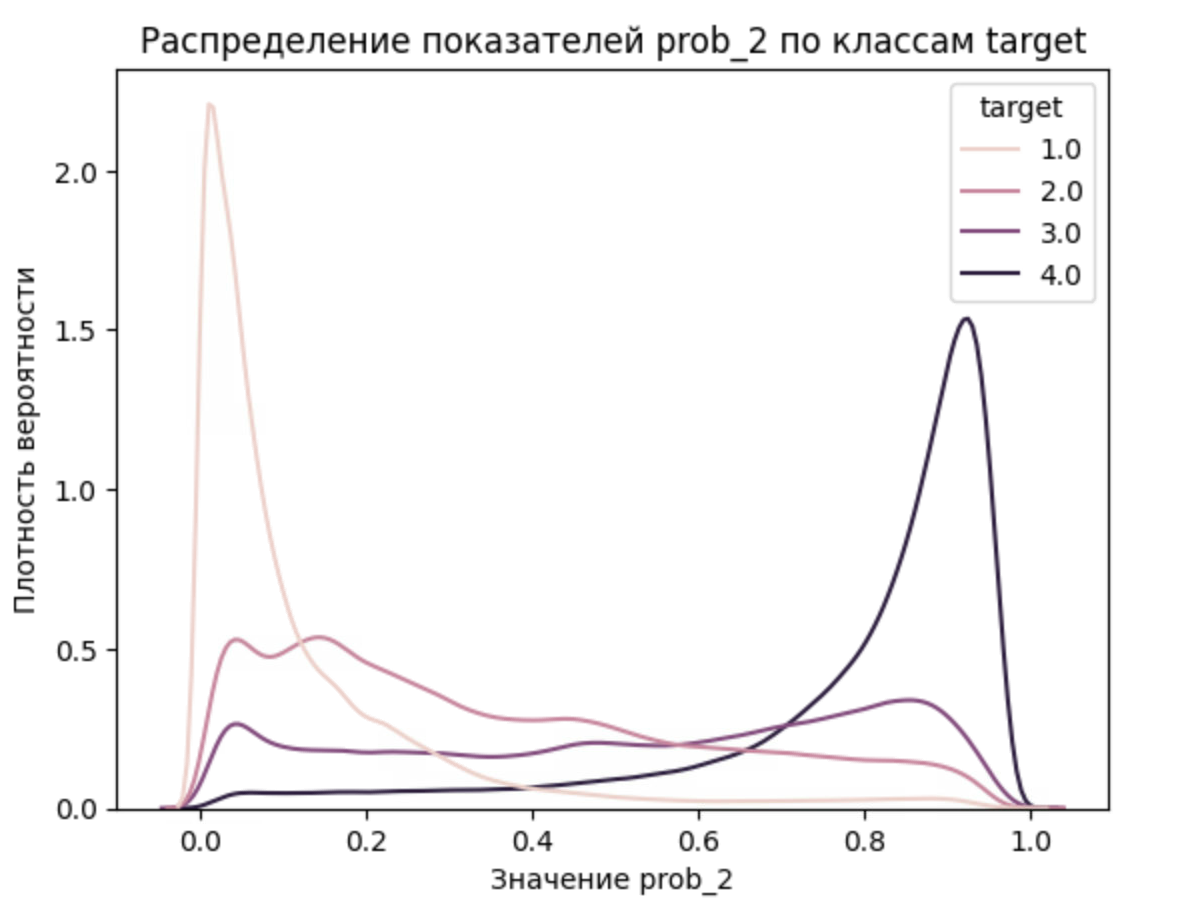
\includegraphics[width=0.9\textwidth]{../figures/prob_2_our.png}
	\caption{Вероятность выживания в август 2024 для нашей модели}
\end{figure}

\begin{figure}[H]
	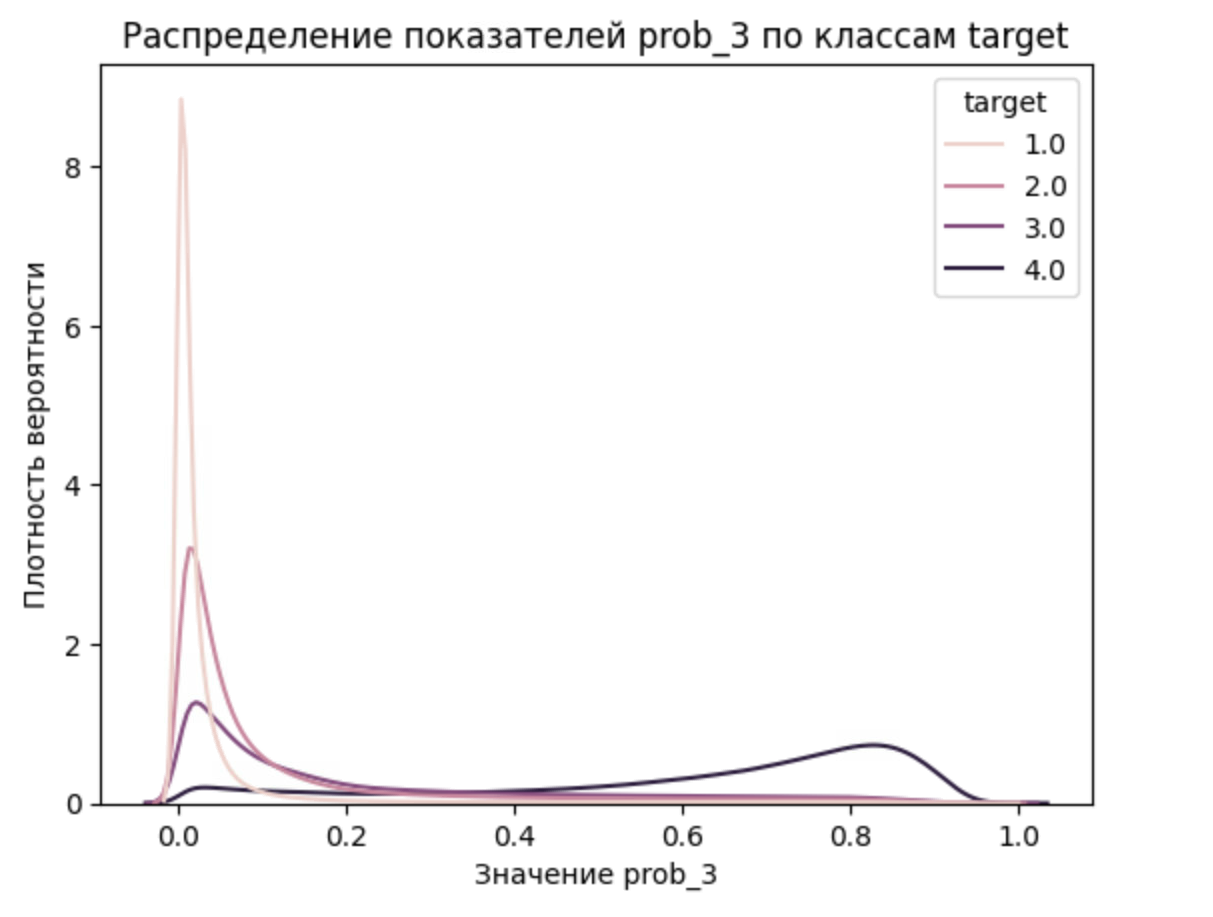
\includegraphics[width=0.9\textwidth]{../figures/prob_3_our.png}
	\caption{Вероятность выживания в сентябрь 2024 для нашей модели}
\end{figure}

Увы, но та же проблема переносится и на нашу модель: оттекшие абоненты имеют схожие графики функций плотностей распределений, поэтому их модель не может адекватно отличить. 



\section{Сравнение различных моделей}

\subsection{Сравнение метрик}

Суммируем все наши данные по метрикам в таблицу:

\begin{table}[H]
	\centering
	\resizebox{\textwidth}{!}{%
		\begin{tabular}{|l|c|l|l|l|}
			\hline
			Название модели                                            & \multicolumn{1}{l|}{Исходная точность} & Точность на 5 признаках                                 & Потеря точности                                        & $C$-индекс                                            \\ \hline
			DeepHit                                                    &                                        & $73.1\%$                                                & $7.5\%$                                                & $0.74$                                                \\ \cline{1-1} \cline{3-5} 
			PMF                                                        &                                        & $75.2\%$                                                & $5.4\%$                                                & $0.75$                                                \\ \cline{1-1} \cline{3-5} 
			Nnet-survival                                              &                                        & $74.8\%$                                                & $5.8\%$                                                & $0.77$                                                \\ \cline{1-1} \cline{3-5} 
			\cellcolor[HTML]{FE0000}{\color[HTML]{000000} Наша модель} & \multirow{-4}{*}{$80.6\%$}             & \cellcolor[HTML]{FE0000}{\color[HTML]{000000} $78.5\%$} & \cellcolor[HTML]{FE0000}{\color[HTML]{000000} $2.1\%$} & \cellcolor[HTML]{FE0000}{\color[HTML]{000000} $0.81$} \\ \hline
		\end{tabular}%
	}
\end{table}

Как видно, наша модель превосходит остальные модели.

\subsection{Вывод по интерпретации вероятностей выживания}

Что касается результатов отдения отточников между собой - тут результаты более удручающие. По результатам обсуждения данного результата внутри Мегафона было выяснено, что данная причина связана с низкой изменчивостью клиентских данных за месячный период. Из за этого задача классификации и отделения отточников, которые оттекают в соседние месяцы является в Мегафоне тяжелой задачей, даже для хорошо зарекомендовавших себя моделей градиентного бустинга. 

\section{Наша модель на расширенном датасете}

Как было написано выше, наша модель, как и все остальные, довольно плохо отличает отточников друг от друга. Тогда возникла гипотеза, что если увеличить обучающую выборку, добавив в нее больше месяцев, то модель сможет лучше научиться отличать отточников. Получились следующие графики плотностей вероятностей: 

\begin{figure}[H]
	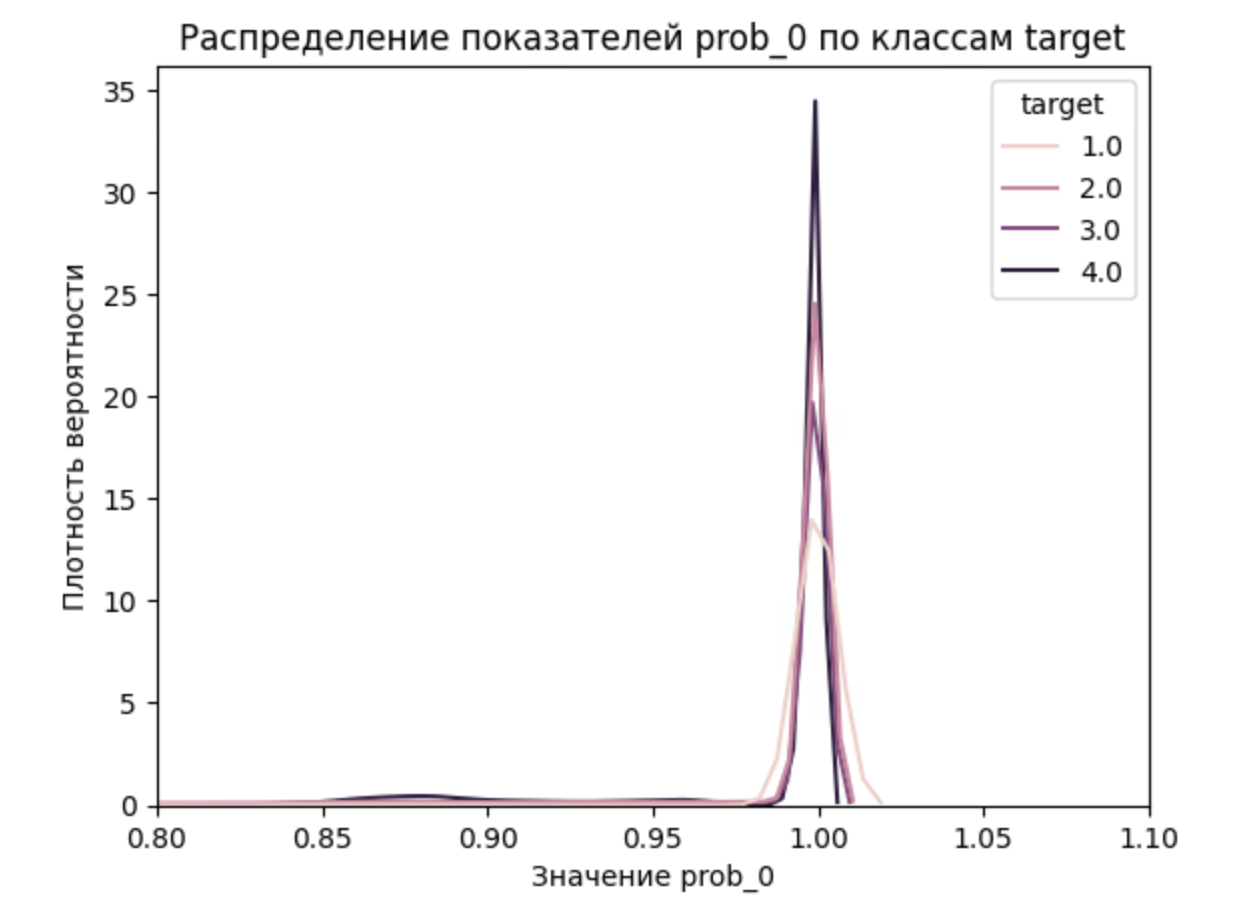
\includegraphics[width=0.9\textwidth]{../figures/prob_0_ours.png}
	\caption{Вероятность выживания в январь 2024 для нашей модели}
\end{figure}

\begin{figure}[H]
	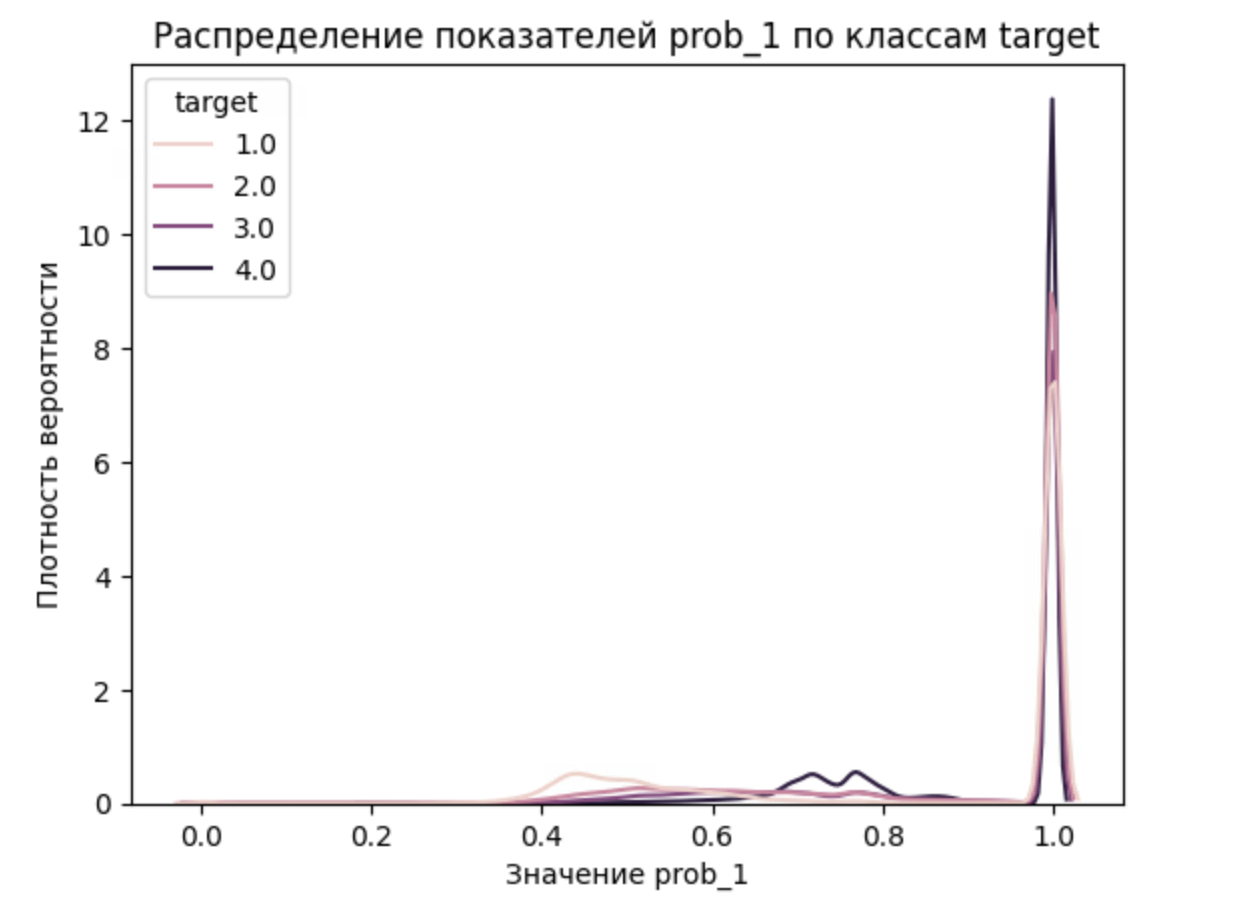
\includegraphics[width=0.9\textwidth]{../figures/prob_1_ours.png}
	\caption{Вероятность выживания в февраль 2024 для нашей модели}
\end{figure}

\begin{figure}[H]
	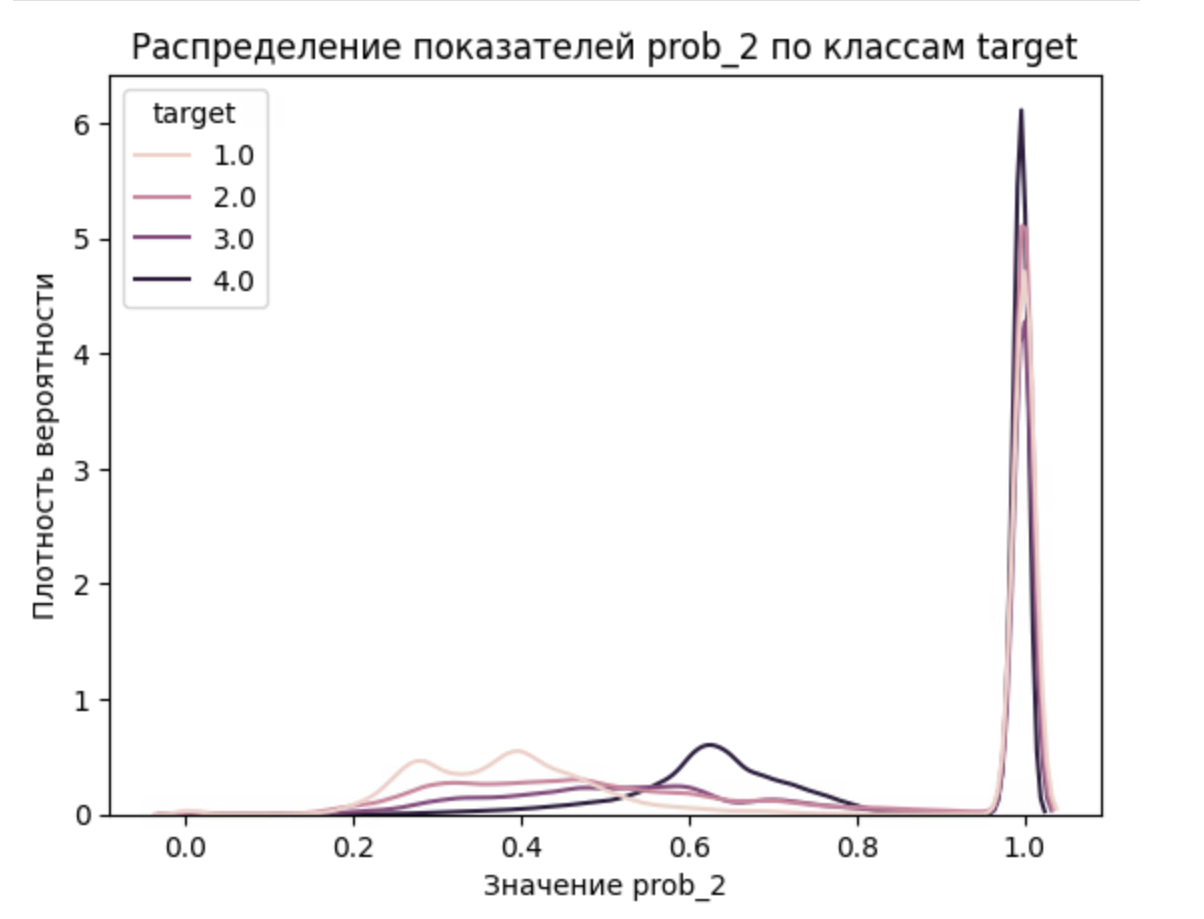
\includegraphics[width=0.9\textwidth]{../figures/prob_2_ours.png}
	\caption{Вероятность выживания в март 2024 для нашей модели}
\end{figure}

\begin{figure}[H]
	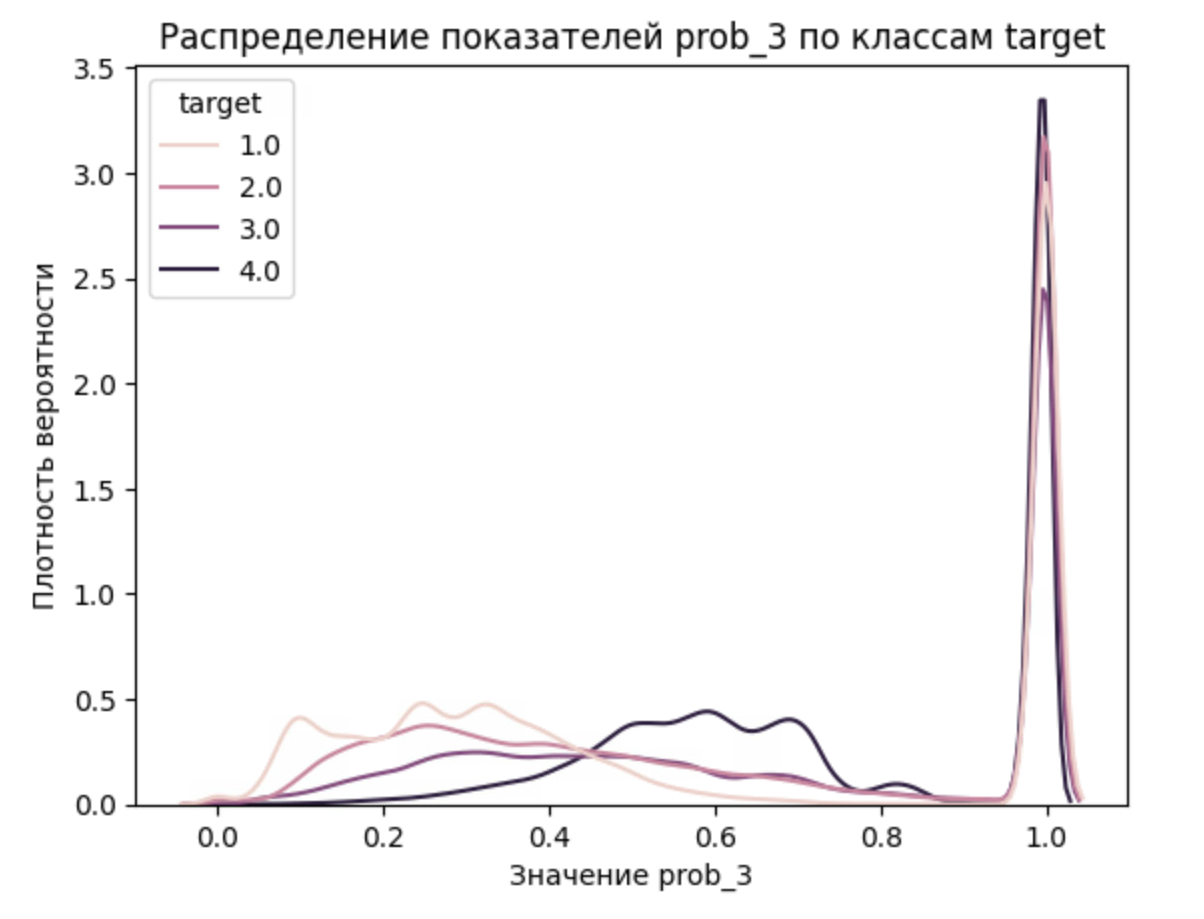
\includegraphics[width=0.9\textwidth]{../figures/prob_3_ours.png}
	\caption{Вероятность выживания в апрель 2024 для нашей модели}
\end{figure}

\begin{figure}[H]
	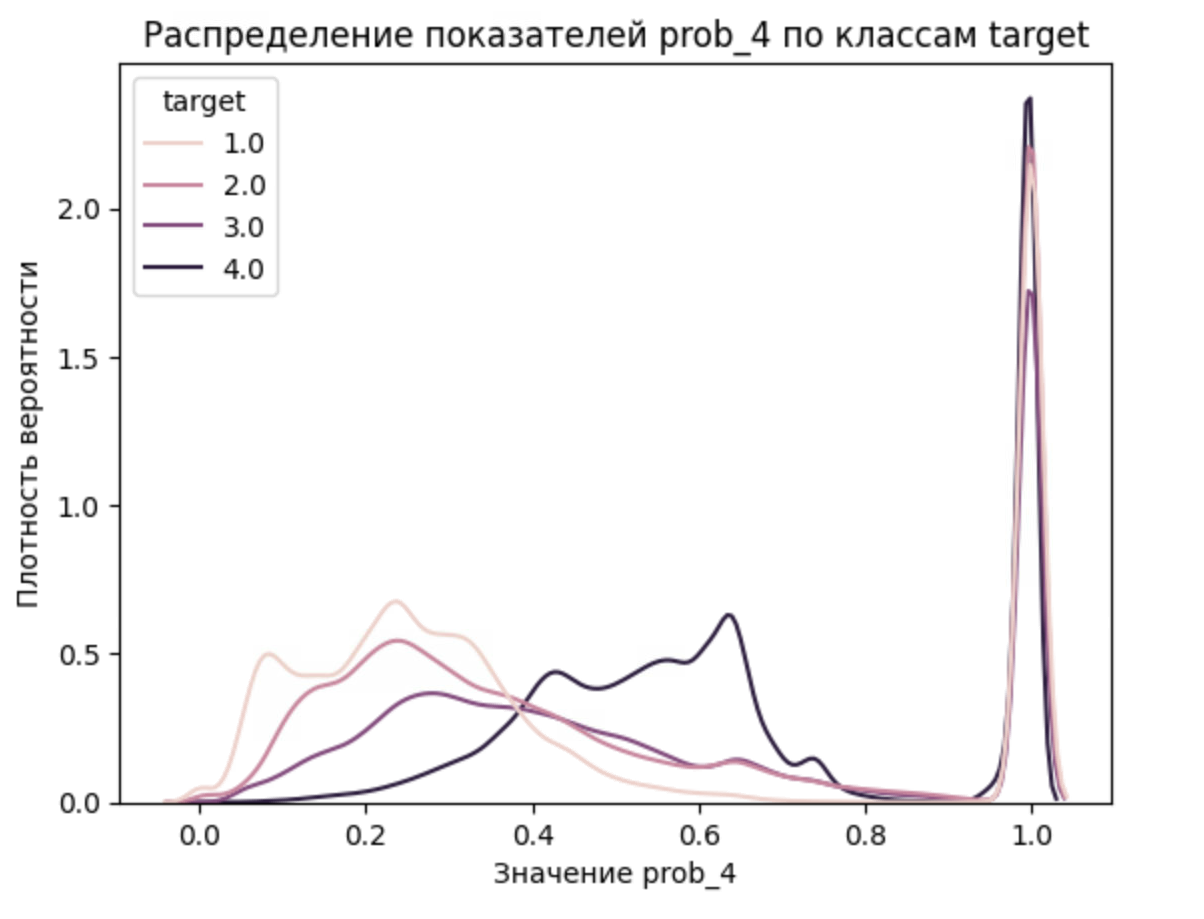
\includegraphics[width=0.9\textwidth]{../figures/prob_4_ours.png}
	\caption{Вероятность выживания в май 2024 для нашей модели}
\end{figure}

\begin{figure}[H]
	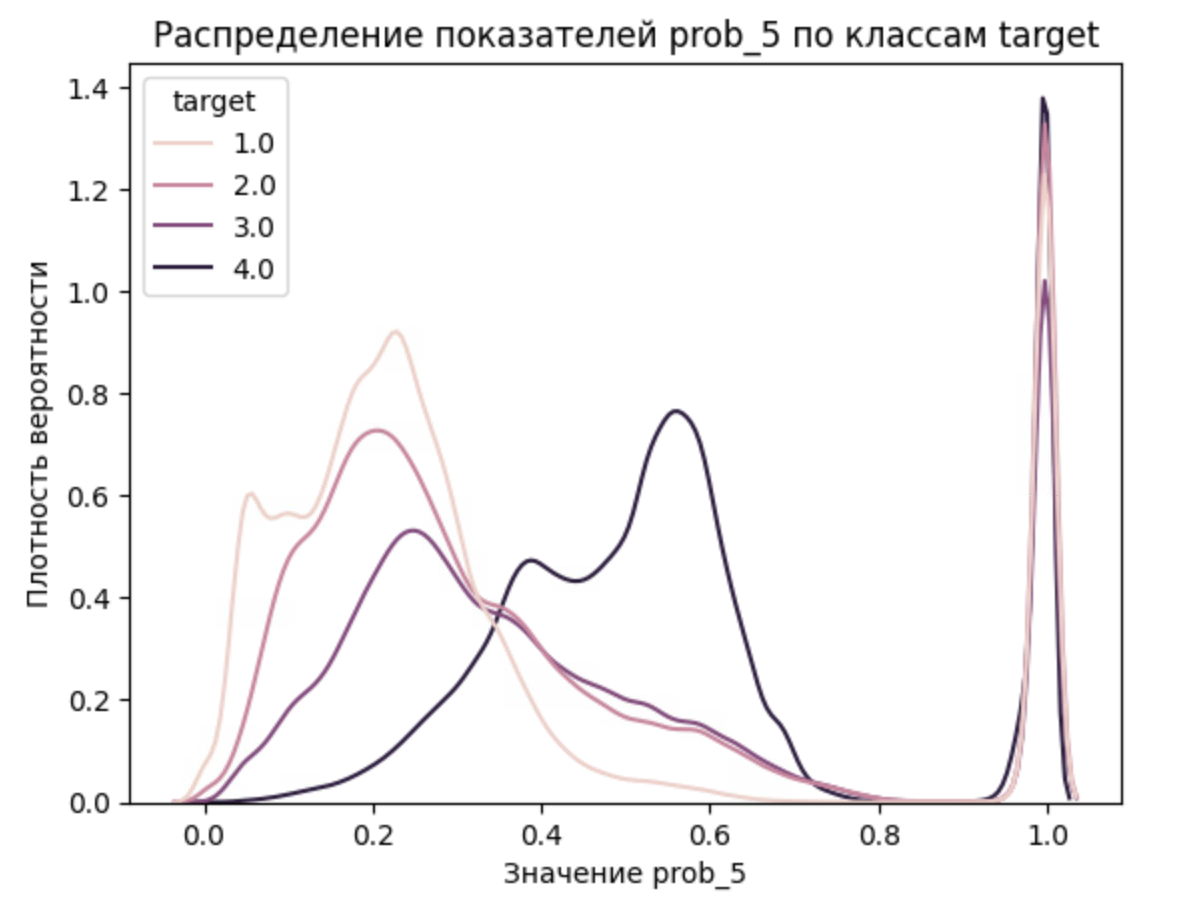
\includegraphics[width=0.9\textwidth]{../figures/prob_5_ours.png}
	\caption{Вероятность выживания в июнь 2024 для нашей модели}
\end{figure}

\begin{figure}[H]
	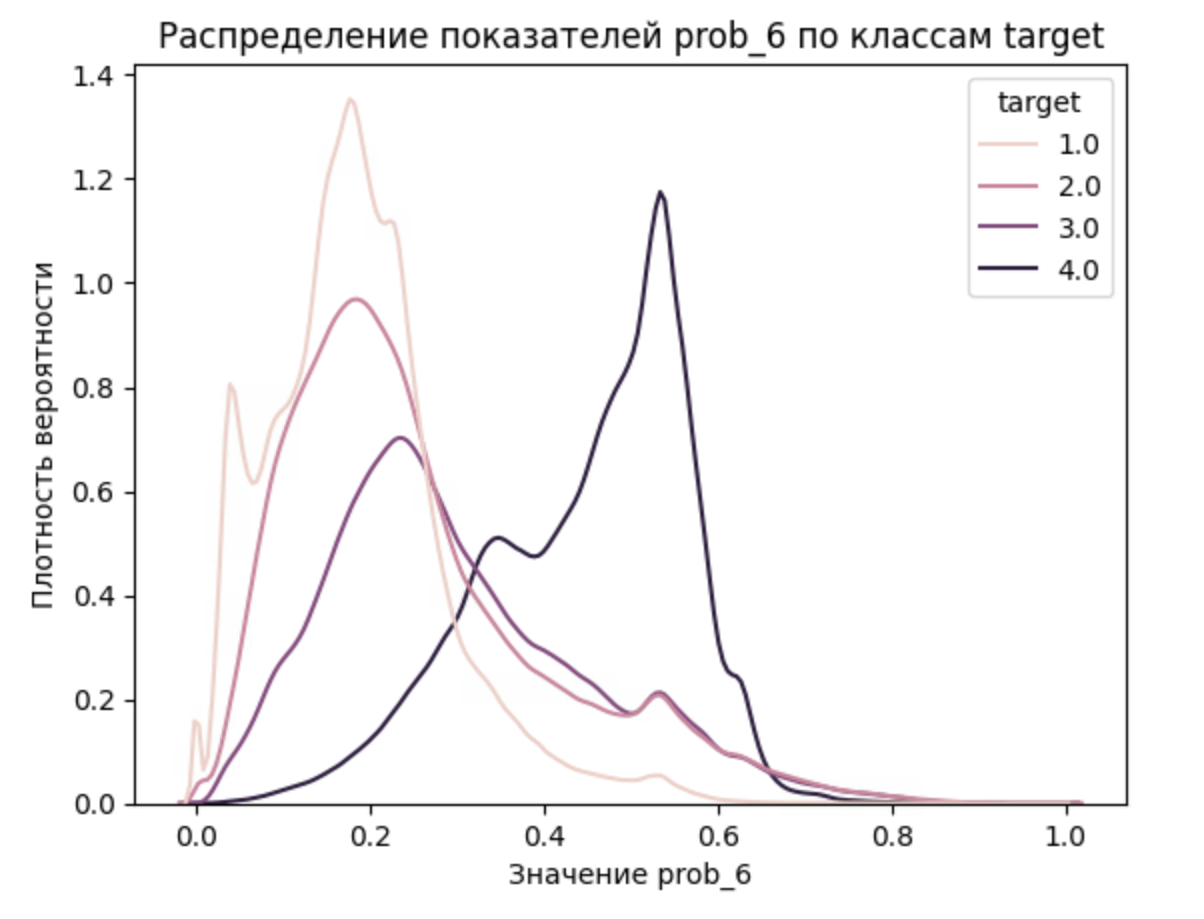
\includegraphics[width=0.9\textwidth]{../figures/prob_6_ours.png}
	\caption{Вероятность выживания в июль 2024 для нашей модели}
\end{figure}

\begin{figure}[H]
	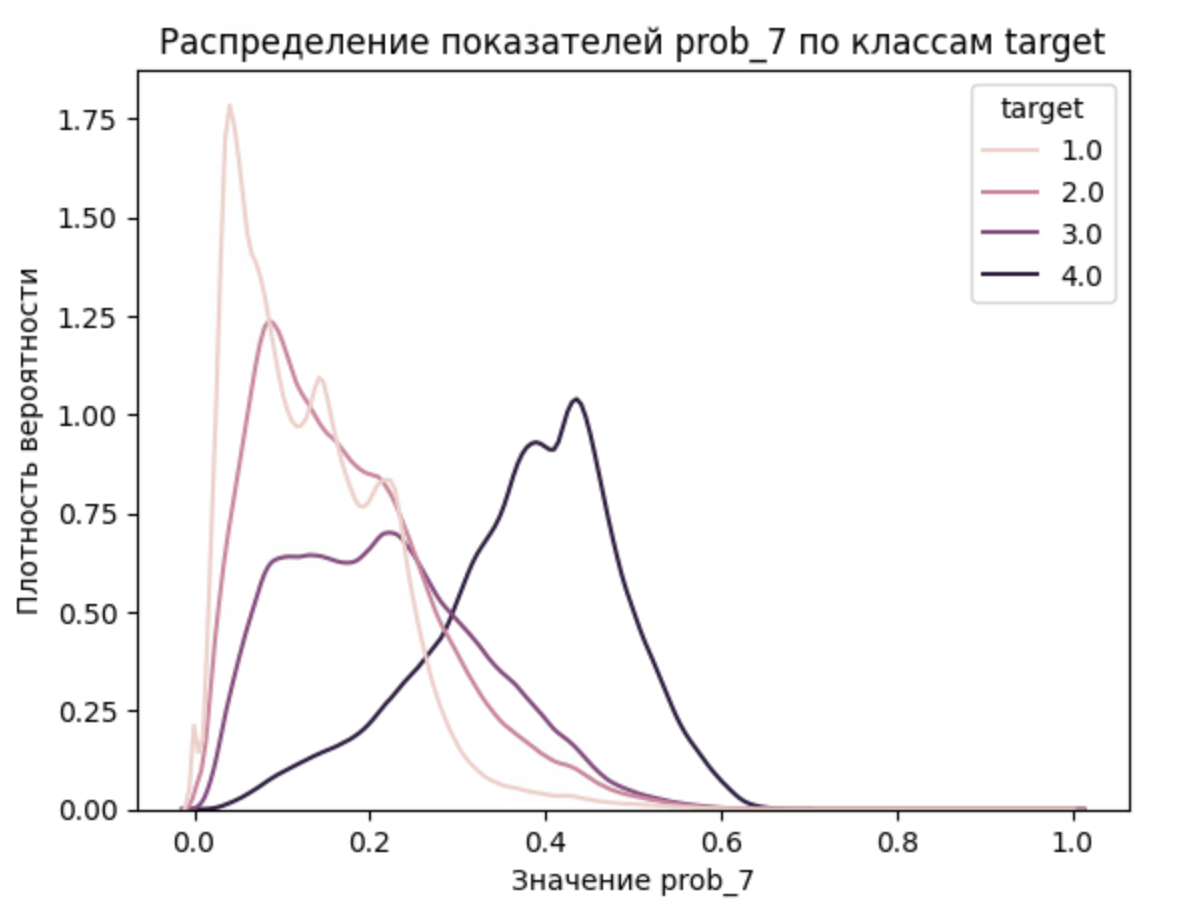
\includegraphics[width=0.9\textwidth]{../figures/prob_7_ours.png}
	\caption{Вероятность выживания в август 2024 для нашей модели}
\end{figure}

\begin{figure}[H]
	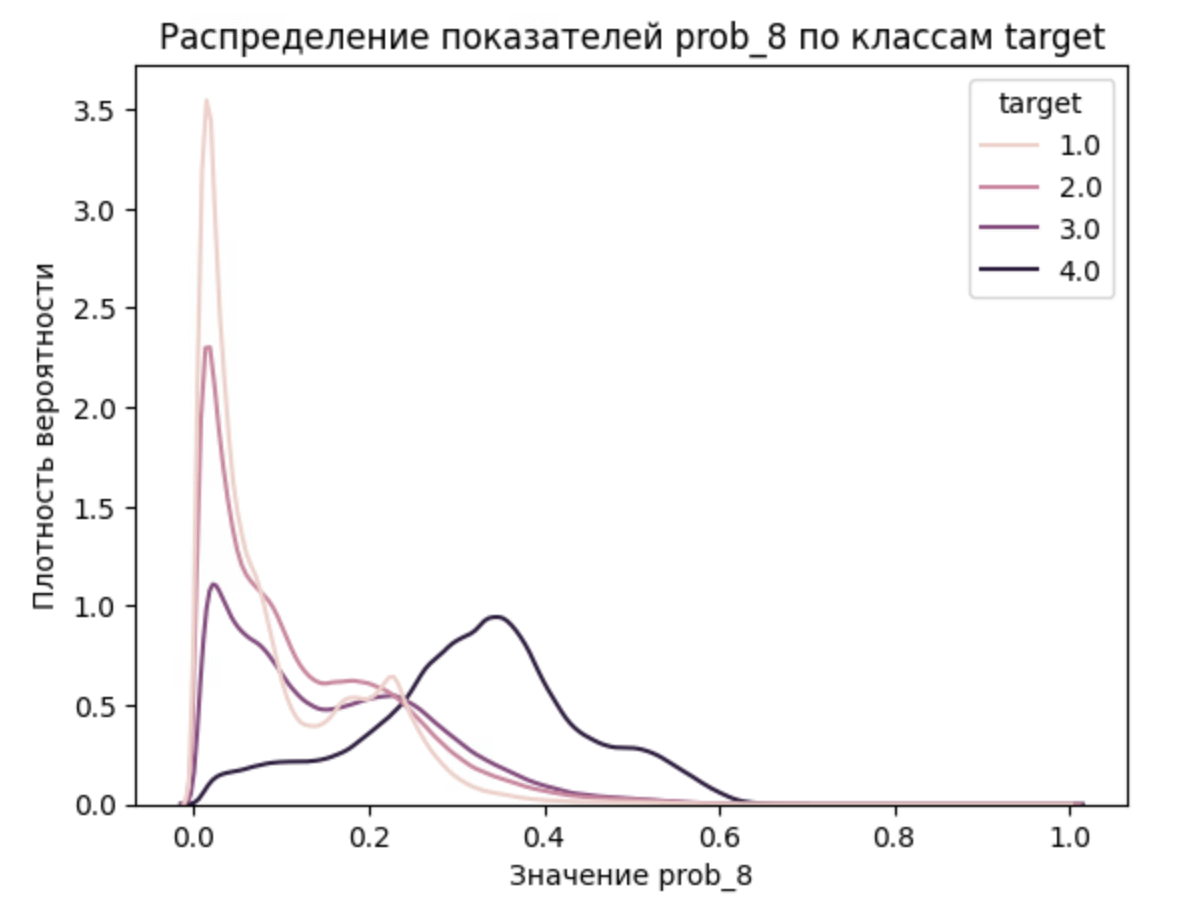
\includegraphics[width=0.9\textwidth]{../figures/prob_8_ours.png}
	\caption{Вероятность выживания в сентябрь 2024 для нашей модели}
\end{figure}

\begin{figure}[H]
	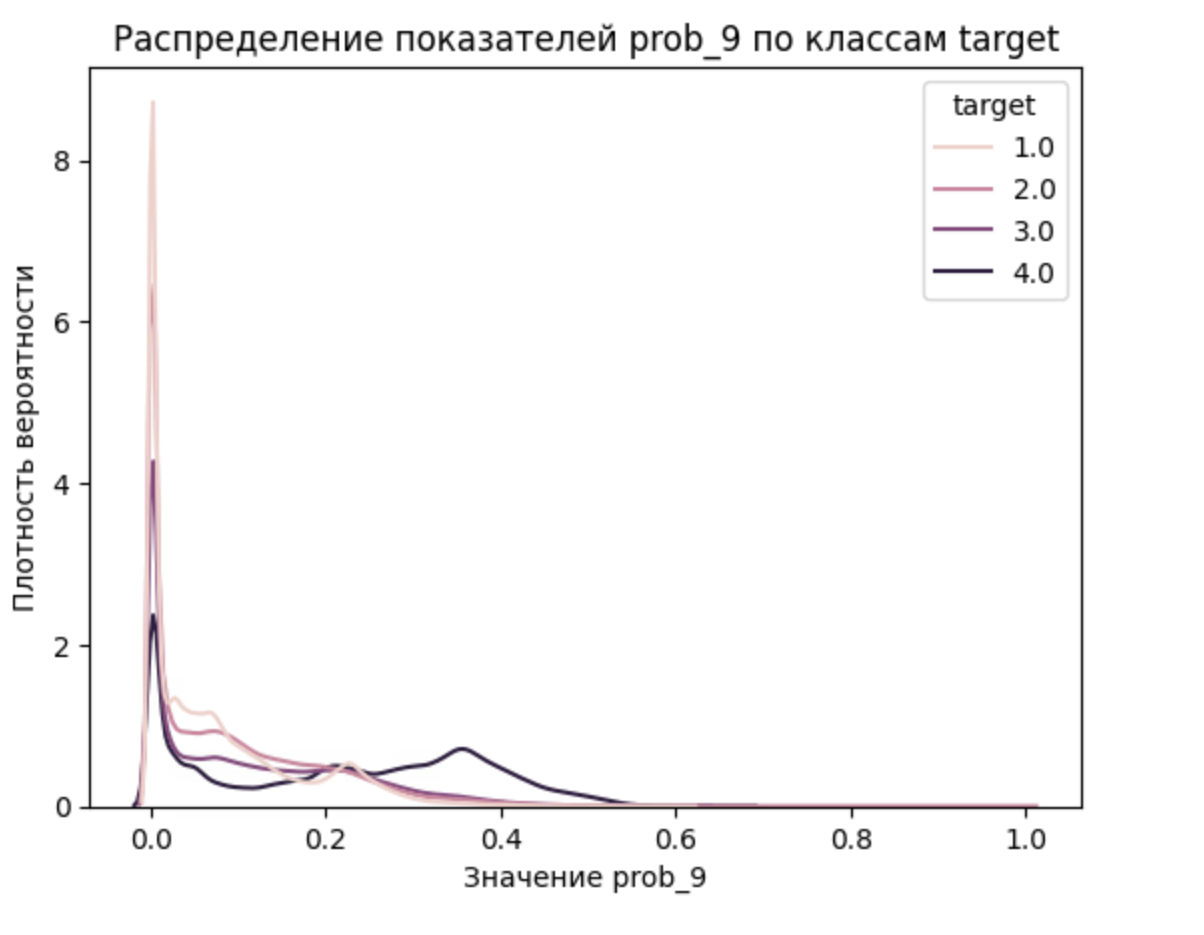
\includegraphics[width=0.9\textwidth]{../figures/prob_9_ours.png}
	\caption{Вероятность выживания в октябрь 2024 для нашей модели}
\end{figure}

Увы, но все таки расширение датасета не помогло решить проблему с отдением отточников - мы видим из графиков, что плотности вероятностей для таргетов 1-3 довольно близки друг к другу. Объясняется это тем же свойством датасета - медленным изменением признакового описания абонентов в течении месяца, а также тем, что более прошлая информация о поведении абонента не так сильно влияет на его сегодняшний отток. 


\introchapter{Заключение}

В работе проведен анализ существующих решений из моделей анализа выживаемости, кратко описаны их отличия и проведены сравнения данных моделей на задаче оттока клиентов Мегафона.

В рамках работы была разработана модель, отличающаяся от предыдущих использованием временных рядов векторов признаков. Архитектура модели состоит из RNN блока, механизма внимания и перцептрона и является известным и хорошо зарекомендовавшим себя решением в моделях выживания. Основная новизна работы заключается в использовании специфической функции потерь. В работе доказывается свойство добавки к функции потерь.

Модель, разработанная в данной работе, показала более высокие результаты по сравнению с другими моделями в плане более низкой потери качества на "сжатом" признаковом описании и более высоким $C$-индексом. К сожалению, наша модель не смогла решить проблему с классификацией отточников, хотя она и хорощо отделяет отточников от сохраняющихся абонентов, как и остальные модели.

Основным направлением дальнейших исследований можно выделить решение проблемы с классификацией отточников. Здесь автор видит основное решение в более продвинутом использовании Feature Engineering, так как, как показали исследования, корень проблем кроется в медленном изменении клиентских данных. Благо анализ существующих работ позволил выявить множество идей признаков, которые хорошо показали себя у других исследователей и которые могут дать весовый прирост на качество моделей Мегафона.  


%% Настройки библиографии
\bibliographystyle{gost71u}
\nocite{*}
\bibliography{references}


\end{document}